% Capítulo 3 - Metodología, Experimentación y Resultados 
\chapter{Metodología, Experimentación y Resultados}
\label{cap:Metodologia}
Este capítulo detalla el núcleo práctico y experimental del presente Trabajo de Fin de Máster. A lo largo de las siguientes secciones, se describe exhaustivamente la metodología aplicada para abordar la detección y clasificación del discurso sexista en redes sociales. En primer lugar, se contextualiza el marco del proyecto dentro del desafío de \textit{EXIST 2025}. A continuación, se expone el pipeline de preparación de los datos y se desglosan los experimentos realizados de forma unimodal (abarcando el procesamiento de texto, imágenes estáticas y secuencias de vídeo). Finalmente, se detalla la integración de estas arquitecturas mediante técnicas de fusión multimodal, culminando con un análisis profundo sobre el perspectivismo de los datos y la presentación de los resultados globales obtenidos. 

\section{Participación en el desafío \textit{EXIST 2025}}
\label{sec:ParticipacionDesafioEXIST2025}
El presente trabajo se ha desarrollado en el marco del desafío internacional \textit{EXIST 2025} (\textit{sEXism Identification in Social neTworks}). Esta iniciativa tiene como objetivo principal pedir a los participantes que identifiquen y caractericen el sexismo en las redes sociales. Su propósito fundamental es ayudar a identificar tendencias y patrones de comportamiento sexista en diversos formatos multimedia y de interacción de usuarios, contribuyendo así a una comprensión más profunda de estas dinámicas sociales y a su potencial aplicabilidad en sistemas de moderación de contenido. 

\subsection*{Estructura del reto y modalidades}
\label{subsec:EstructuraDelRetoYModalidades}
En su edición de 2025, la organización ha dado un salto cualitativo hacia la multimodalidad, conformando un total de nueve subtareas disponibles en dos idiomas (inglés y español). Estas subtareas se estructuran en torno a tres ejes principales (Identificación de sexismo, Detección de la intención de la fuente y Categorización del sexismo) aplicadas a tres tipos de datos diferentes:
\begin{itemize}
    \item \textbf{Tarea 1 (Texto)}: Centrada en el análisis de \textit{tweets}.
    \item \textbf{Tarea 2 (Imágenes)}: Enfocada en la evaluación de memes, extrayendo su información visual y textual mediante \textit{OCR}.
    \item \textbf{Tarea 3 (Vídeos)}: Basada en archivos multimedia extraídos de la plataforma \textit{TikTok}.
\end{itemize}

Esta aproximación multimodal resulta esencial para evaluar la capacidad real de los sistemas a la hora de detectar la subjetividad y la ofensa en fuentes de datos complejas.

\subsection*{Participación global y datos del reto}
\label{subsec:ParticipacionGlobalYDatosDelReto}
La relevancia de esta edición quedó demostrada por un nivel de implicación excepcional en la comunidad científica. Un total de 244 equipos de 38 países se registraron en \textit{EXIST 2025}, de los cuales 114 (procedentes de 23 países) lograron enviar al menos una entrega (\textit{run}) oficial. En conjunto, se recibieron 873 envíos, de los cuales 589 se evaluaron mediante \textit{Hard-labels} y 284 mediante \textit{Soft-labels}.

Aunque la mayoría de los participantes concentraron sus esfuerzos en el análisis puramente textual de la Tarea 1 (596 envíos evaluados), la Tarea 3 dedicada al análisis de vídeo atrajo un interés significativo con 211 envíos, lo que subraya la creciente relevancia de los enfoques multimodales en el PLN. 

\subsection*{Nuestras entregas oficiales y motivación del TFM}
\label{subsec:NuestrasEntregasOficialesYMotivacionDelTFM}
En el contexto oficial del desafío, la participación de nuestro equipo (\textit{I2C-UHU}) se enmarcó dentro de la Tarea 3 de vídeos, concretamente en la \textbf{Subtarea 3.1 (Identificación de Sexismo)}. Se trata de un problema de clasificación binaria donde el sistema debe decidir si un contenido dado refleja expresiones o comportamientos sexistas, clasificándolo bajo las categorías ``YES'' o ``NO''.

Para nuestras dos entregas oficiales, se optó por un enfoque inicial unimodal, evaluando la capacidad de la transcripción textual del vídeo para resolver la tarea. Se realizaron los siguientes envíos bajo la evaluación \textit{Hard}:
\begin{enumerate}
    \item \textbf{I2C-UHU-Sirius\_1}: Un modelo discriminativo de la familia \textit{Transformer} (\texttt{bert} \texttt{-base-multilingual-cased}), ajustado mediante \textit{fine-tuning} para la clasificación de secuencias.
    \item \textbf{I2C-UHU-Sirius\_2}: Un \textit{LLM} generativo (\texttt{meta-llama/Llama-3.2-1B-Instruct}), evaluado bajo un enfoque \textit{Zero-Shot} mediante técnicas de \textit{Prompt Engineering}.  
\end{enumerate}

En la \autoref{tab:ResultadosOficialesEXIST} se detallan las métricas oficiales obtenidas por nuestros sistemas en la evaluación oficial sobre un total de 43 participaciones admitidas en la tabla de clasificación (\textit{leaderboard}) para esta subtarea. Cabe destacar que estas métricas oficiales basadas en \textit{ICM-Hard} y el \textit{F1} de la clase \textit{YES} responden a un protocolo específico (el definido por la organización) y no son directamente comparables con los resultados locales obtenidos en fases posteriores de este trabajo (medidos habitualmente mediante \textit{macro-F1}).

\begin{table}[H]
    \centering
    \begin{tabular}{lcccc}
        \toprule
        \textbf{Envío Oficial} & \textbf{Ranking} & \textbf{ICM-Hard} & \textbf{ICM-Hard Norm} & \textbf{F1 Macro} \\
        \midrule
        (\textit{BERT}) & 31 & -0.1278 & 0.4355 & 0.5768 \\
        (\textit{LLaMA}) & 39 & -0.4212 & 0.2874 & 0.1379 \\
        \bottomrule
    \end{tabular}
    \caption{Resultados oficiales obtenidos en la Subtarea 3.1 de EXIST 2025}
    \label{tab:ResultadosOficialesEXIST}
\end{table}

Lejos de ser el objetivo final de esta investigación, la participación en el desafío y los resultados expuestos actuaron como el \textbf{\textit{baseline}} de este Trabajo de Fin de Máster. Las métricas alcanzadas (en especial el bajo rendimiento del enfoque \textit{Zero-Shot}) permiten plantear la hipótesis de que la restricción metodológica a un formato exclusivamente textual (sumada a factores simultáneos como el tamaño del modelo, el diseño del \textit{prompt}, la ausencia de ajuste fino y la naturaleza específica del conjunto de validación) pudo influir en los resultados. Esta comprobación preliminar sirvió de base para motivar y justificar el posterior trabajo empírico, desarrollado en esta memoria: la extracción de fotogramas, la experimentación profunda con modelos de visión estática y temporal, la integración mediante \textit{Ensembles} y el análisis de la subjetividad de los anotadores.

\section{Descripción General de la Metodología}
\label{sec:Metodologia}

\begin{figure}[H]
    \centering
    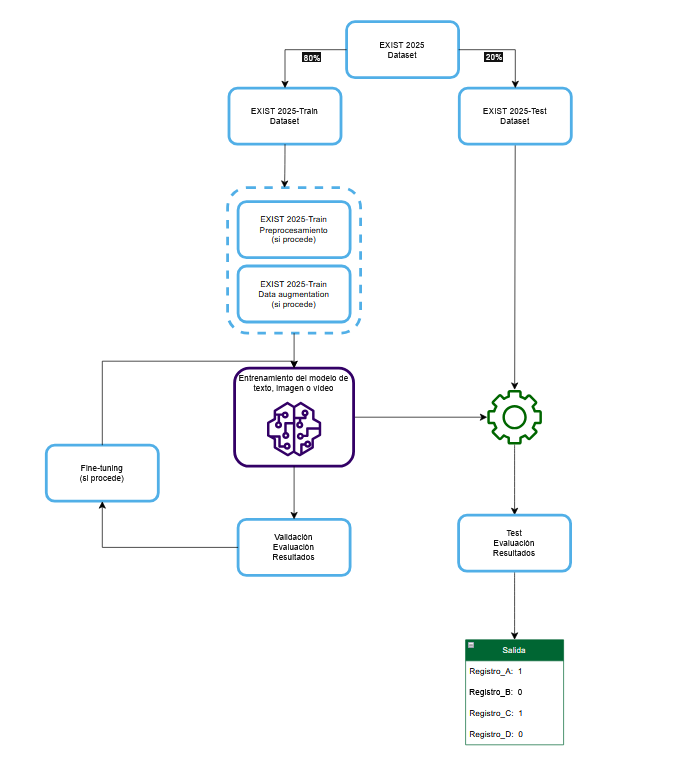
\includegraphics[width=0.9\textwidth]{Figuras/PipelineSeguida.png}
    \caption{Pipeline general del marco de experimentación}
    \label{fig:PipelineSeguida}
\end{figure}

El marco de experimentación diseñado para este Trabajo de Fin de Máster se ha dividido en un flujo de trabajo iterativo e incremental: comenzando por el preprocesamiento de los datos, pasando por el diseño y entrenamiento de modelos unimodales, y culminando con la fusión multimodal y la evaluación del rendimiento bajo diferentes perspectivas. En esta sección se ofrece una visión general del proceso completo, el cual será detallado en profundidad en secciones posteriores. 

La \autoref{fig:PipelineSeguida} muestra el \textit{pipeline} del marco de experimentación seguido en este trabajo. 

De forma estructurada, la secuencia completa de procesos abordada para resolver la detección y categorización del discurso sexista se divide en las siguientes fases principales:
\begin{enumerate}
    \item \textbf{Preparación y Tratamiento de Datos}: Esta fase inicial engloba la limpieza del corpus textual y la estandarización del conjunto de datos mediante una división estratificada. Se generó un conjunto de \textit{Train} y un \textit{Test} local de desarrollo (destinado empíricamente a la calibración y selección de modelos). Para garantizar una reproducibilidad estricta, los identificadores exactos (\textit{IDs}) de los vídeos pertenecientes a cada partición se han publicado en el repositorio del proyecto. Finalmente, se llevó a cabo la extracción automatizada de características visuales, procesando los archivos multimedia para generar diferentes conjuntos de \textit{frames}.
    \item \textbf{Selección y Entrenamiento Unimodal}: Ante la complejidad del formato vídeo, se optó por la estrategia de ``divide y vencerás'', seleccionando y entrenando arquitecturas expertas para cada modalidad de forma aislada:
    \begin{itemize}
        \item \textit{Modalidad de texto}: Experimentación con modelos discriminativos multilingües (familia \textit{Transformer}) y modelos generativos masivos (\textit{LLMs}).
        \item \textit{Modalidad de Visión Estática y Temporal}: Ajuste de modelos convolucionales de imágenes y redes especializadas en vídeo para captar el contexto visual del problema.
    \end{itemize}
    \item \textbf{Ajuste de Hiperparámetros}: Proceso crítico aplicado a los mejores modelos base seleccionados en la fase anterior. Implicó la exploración del espacio de hiperparámetros (\textit{learning rate}, \textit{weight decay}, \textit{warmup}) para lograr un \textit{fine-tuning} estable, evitando el olvido catastrófico del conocimiento previo de las redes. 
    \item \textbf{Fusión Multimodal (\textit{Ensemble})}: Etapa de consolidación donde las predicciones aisladas de los modelos de texto, imagen y vídeo se combinaron en un único sistema robusto mediante una estrategia de \textit{Late Fusion}, optimizando matemáticamente los pesos de cada modalidad para la Tarea 3.1.
    \item \textbf{Perspectivismo y Análisis de Errores}: Aprovechando el \textit{LeWiDi} del conjunto de datos original, se volvieron a entrenar las mejores arquitecturas de la modalidad de texto segmentando los datos en función del género de los anotadores (perspectiva de hombres frente a mujeres) y se inyectaron roles en los \textit{LLMs} mediante \textit{Persona Prompting} para analizar la subjetividad de los fallos del sistema.  
    \item \textbf{Evaluación y Experimentación Multietiqueta}: Fase final orientada a cuantificar el rendimiento mediante métricas estándar sobre los conjuntos estáticos y a adaptar los mejores modelos unimodales para resolver el problema secundario de la Tarea 3.3 (clasificación independiente de las distintas categorías del sexismo). 
\end{enumerate}

\section{Preparación de los Datos}
\label{Preparacion_Datos}
El rendimiento de los modelos de \textit{deep learning} depende de la calidad y el formato de los datos con los que son entrenados. Por ello, antes de proceder a la fase de modelado, se diseñó un riguroso \textit{pipeline} de preparación. Esta sección detalla la exploración inicial del conjunto proporcionado, la resolución de conflictos con las etiquetas, el preprocesado de las transcripciones textuales y la extracción estructurada de las características visuales a partir de los vídeos originales. 

\subsection{Descripción del Conjunto de Datos y División (\textit{Train} y \textit{Test})}
\label{DescripciónDelConjuntoDeDatosYDivisionTrainYTest}
\begin{figure}[H]
    \centering
    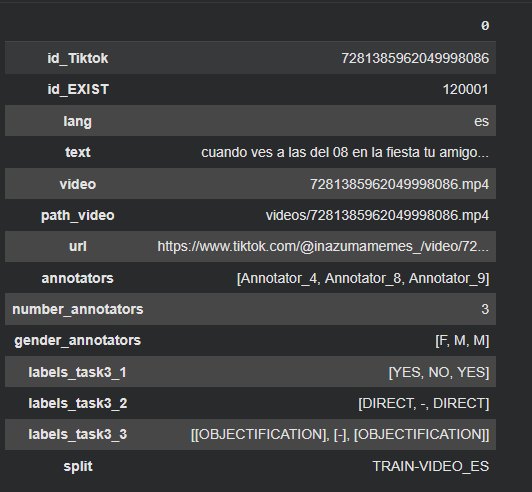
\includegraphics[width=0.9\textwidth]{Figuras/DatasetOriginal.png}
    \caption{Ejemplo de un registro del dataset original}
    \label{fig:DatasetOriginal}
\end{figure}

El conjunto de datos original proporcionado por la organización para la Tarea 3 estaba compuesto por 2524 vídeos extraídos de la plataforma \textit{TikTok} (1524 en español y 1000 en inglés). Estos datos se encontraban estructurados en un archivo \textit{JSON} donde los campos más relevantes para nuestra tarea eran el identificador (\texttt{id\_EXIST}), el texto (\texttt{text}), la ruta del archivo (\texttt{path\_video}), el recuento de los anotadores (\texttt{number\_annotators}) y la lista de valoraciones (\texttt{labels\_task3\_1}). Al basarse en el paradigma de \textit{LeWiDi}, los vídeos no contaban con una etiqueta única, sino que presentaban las decisiones individuales de 2 o 3 anotadores distintos, tal y como se puede observar en la \autoref{fig:DatasetOriginal}.

Para adaptar este conjunto a los requisitos de la Tarea 3.1 (clasificación binaria \textit{Hard} en ``YES'' o ``NO'') era necesario fusionar las múltiples opiniones en una única etiqueta. Según la documentación oficial del reto, el proceso de anotación contemplaba la participación de dos anotadores independientes y la intervención de un investigador experto para adjudicar y resolver los casos de desacuerdo. Al explorar el campo \texttt{labels\_task3\_1}, se verificó que la presencia de un tercer voto correspondía a la inclusión de este veredicto de desempate. 

Dado que el archivo en bruto proporcionado no exponía de forma explícita una columna con la etiqueta \textit{Gold Standard} unificada, se optó por ignorar el supuesto \textit{label} oficial externo y reconstruir las etiquetas desde las matrices de votación para asegurar la coherencia absoluta del conjunto de entrenamiento:
\begin{itemize}
    \item \textbf{Voto por mayoría}: En la inmensa mayoría de las instancias, que contaban con 3 anotadores (reflejando la adjudicación),se asignó directamente la etiqueta mayoritaria. Por ejemplo: un registro con los votos \texttt{[YES, NO, YES]} se catalogó de forma automática como sexista.
    \item \textbf{Descarte por conflicto}: Durante el procesamiento de las etiquetas, se aplicó un \textbf{criterio} estricto de exclusión para aquellos casos en los que no se llegó a un consenso. Específicamente, se detectaron 16 casos residuales evaluados únicamente por 2 anotadores en los que existía un empate absoluto (1 voto a favor y 1 en contra), sin constancia de un tercer voto de resolución en la matriz de datos. En lugar de forzar una asignación de manera manual o aleatoria, se eliminaron estas muestras. El \textbf{impacto} estadístico de esta decisión supone una reducción marginal del corpus (eliminando apenas un 0.8\% de los datos, para fijar el conjunto final de entrenamiento en 2006 instancias), pero resulta metodológicamente crítico para evitar inyectar ruido e inconsistencias en la red neuronal. Para garantizar la trazabilidad de esta limpieza, los identificadores de estas muestras han sido documentados \footnote{Los \textit{IDs} de los 16 vídeos descartados por empate absoluto son: [120157, 120165, 120478, 120551, 120785, 120997, 121304, 121316, 220023, 220157, 220778, 220793, 220872, 220921, 220929, 121443]}.

\end{itemize}

Para asegurar la total reproducibilidad de esta reducción, el filtro se ejecutó automáticamente mediante un \textit{script} incluido en el cuaderno \texttt{Dataset\_Task\_3\_1.ipynb}. Tras aplicarlo, tal y como se puede apreciar en la \autoref{fig:Dataset3.1Transformado}, el conjunto original de 2524 vídeos se redujo a 2508 registros limpios (1306 no sexistas y 1202 sexistas), garantizando que los modelos se entrenaran exclusivamente sobre instancias con un consenso humano verificable.  

\begin{figure}[H]
    \centering
    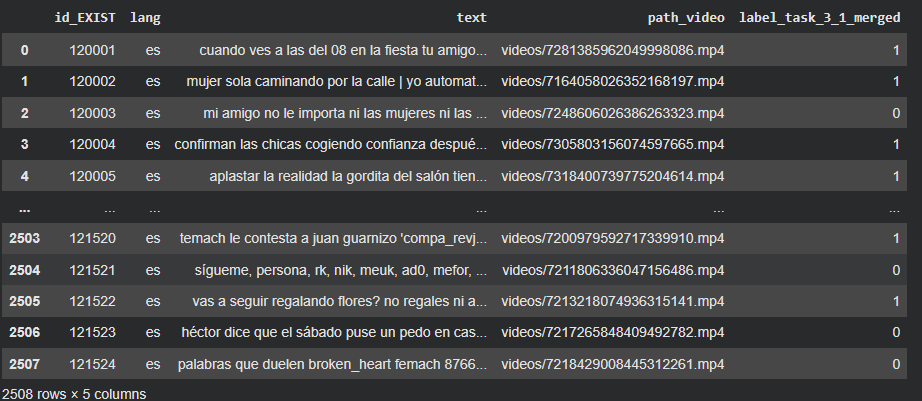
\includegraphics[width=0.9\textwidth]{Figuras/Dataset3.1Transformado.png}
    \caption{Dataset transformado para la tarea 3.1}
    \label{fig:Dataset3.1Transformado}
\end{figure}

Posteriormente, el conjunto consolidado se dividió en dos subconjuntos manteniendo una proporción del 80\% para \textit{Train} y un 20\% para \textit{Test} de validación interna. Se utilizó una técnica de muestreo estratificado (\textit{stratify}) para asegurar que la proporción de clases se mantuviera idéntica en ambos bloques, fijando una semilla aleatoria (\texttt{random\_state=42}) para garantizar la reproducibilidad de la partición. Como se puede observar en la \autoref{tab:distribucionesFichero3.1}, el conjunto de \textit{Train} final quedó conformado por 2006 instancias (1045 negativas, 961 positivas), mientras que el conjunto de \textit{Test} local constó de 502 instancias (261 negativas, 241 positivas). 

Cabe reconocer que esta metodología no reproduce el protocolo empleado por la organización para generar el \textit{Test} ciego oficial, el cual está fundamentado en una partición cronológica y agrupada por autor para evitar sesgos. Por consiguiente, nuestro marco de calibración local asume un riesgo potencial de fuga de información (\textit{data leakage}), ya que vídeos de un mismo autor de \textit{TikTok} podrían quedar repartidos entre entrenamiento y validación. Esto remarca el carácter exploratorio de nuestras métricas locales, haciendo indispensable la evaluación final sobre el entorno de desafío para confirmar la viabilidad del sistema. 

\begin{table}[H]
    \centering
    \begin{tabular}{lccc}
        \toprule
        \textbf{Fichero} & \textbf{Train} & \textbf{Test}\\
        \midrule
        Etiqueta 1 & 961 & 241 \\
        Etiqueta 0 & 1045 & 261 \\
        Total & 2006 & 502 \\
        \bottomrule
    \end{tabular}
    \caption{Distribuciones del fichero \text{Train} y \textit{Test} para la tarea 3.1}
    \label{tab:distribucionesFichero3.1}
\end{table}

\subsection{Preprocesado de texto, limpieza y tokenización}
\label{PreprocesadoDeTextoLimpiezaYTokenizacion}
Las transcripciones automáticas de los vídeos suelen presentar irregularidades gramaticales. Por ello, el \textit{pipeline} de limpieza se diseñó para operar directamente sobre el campo \textit{text} unificando el tratamiento para ambos idiomas (español e inglés). Primero, el texto fue estandarizado transformando los valores nulos y forzando la compatibilidad de tipo \textit{string} para evitar fallos de ejecución. A continuación, tal y como se describió en el marco teórico, se aplicó una tubería secuencial basada en la librería nativa de expresiones regulares (\textit{regex}), siguiendo este orden de ejecución:

\begin{enumerate}
    \item \textbf{Normalización base}: Conversión de toda la cadena de texto a caracteres en minúsculas.
    \item \textbf{Estructuras de transcripción}: Eliminación de prefijos originados por el sistema de captura del reto (ej. borrado literal de los patrones \texttt{``AUDIO:''} y \texttt{``VIDEO:''}).
    \item \textbf{Metadatos web}: Búsqueda y eliminación de enlaces externos (\textit{URLs}).
    \item \textbf{Interacciones sociales}: Supresión de menciones directas a otros usuarios de la red social (patrón \texttt{@usuario}) y limpieza de etiquetas (\textit{hashtags}).
    \item \textbf{Símbolos y ruido}: Borrado de emoticonos (\textit{emojis}), caracteres especiales y puntuaciones atípicas que no aportan significado semántico al clasificador.
\end{enumerate}

Una vez finalizada la limpieza del texto, el proceso de tokenización varió drásticamente en función de la familia de modelos utilizados: 
\begin{itemize}
    \item \textbf{\textit{Transformers}}: Se emplearon los tokenizadores nativos de cada arquitectura (utilizando algoritmos como \textit{WordPiece} para las variantes de \textit{BERT} y \textit{Byte-Pair Encoding} o \textit{BPE} para \textit{RoBERTa}). Para garantizar la uniformidad de los tensores de entrada y optimizar el consumo de memoria de la GPU, se aplicó un truncamiento y rellenado dinámico (\textit{padding}) estableciendo una longitud máxima de secuencia (\textit{max\_length}) de \textbf{[128]} \textit{tokens}. A nivel interno, una frase como ``\textit{El machismo no existe}'' se descompone en tokens elementales y se traduce a un vector numérico estructurado (por ejemplo: \texttt{[101, 235, 14234, 156, ...]}) denominado \texttt{input\_ids}, acompañado de una máscara de atención (\texttt{attention\_mask}).
    \item \textbf{\textit{LLMs}}: Para el \textit{fine-tuning} de modelos como \textit{LLaMA} o \textit{Mistral}, el preprocesamiento exigió la implementación de una técnica de \textit{Prompt Engineering}. Cada transcripción se envolvió en una plantilla estructurada que indicaba explícitamente al modelo su tarea, restringiendo su vocabulario de salida exclusivamente a las palabras ``YES'' o ``NO''.
\end{itemize}

\subsection{Extracción de Características Visuales}
\label{subsec:ExtraccionDeCaracteristicasVisuales}
Para que los modelos de visión por computador pudieran analizar el contenido de \textit{TikTok}, fue necesario transformar los archivos temporales de vídeo (.mp4) en fotogramas estáticos legibles por redes convolucionales. Este proceso se llevó a cabo utilizando la biblioteca de visión artificial \textit{OpenCV}.

Es importante resaltar que la separación de los datos en los subconjuntos \textit{Train} y \textit{Test} descrita en la primera subsección se realizó aislando el identificador único del vídeo \texttt{id\_EXIST} de manera completamente previa a la extracción de imágenes. El script de procesamiento de \textit{frames} operó leyendo de forma aislada los ficheros que ya estaban particionados. Esta metodología actúa como una estrategia robusta de \textit{GroupSplit}, asegurando que no exista fuga de datos (\textit{data leakage}): todos los datos extraídos de un mismo vídeo recaen íntegramente en la misma partición, impidiendo que el modelo sea evaluado con escenas que ya memorizó durante el entrenamiento. 

Con el objetivo de explorar la cantidad óptima de información visual requerida, se construyeron múltiples \textit{datasets} extrayendo un número variable de fotogramas por vídeo: $N \in \{2, 4, 6, 8, 10\}$. En la \autoref{tab:TamañosFicherosFrames} se aprecian los tamaños y distribuciones de los nuevos \textit{corpus} de imagen generados. Para garantizar que las capturas fueran verdaderamente representativas del contenido global y evitar \textit{frames} en negro al inicio o al final del vídeo, se diseñó un algoritmo de muestreo equidistante. La frecuencia o paso de extracción (\textit{step}) se calculó matemáticamente mediante la siguiente ecuación:

\begin{equation}
    step = \left\lfloor \frac{\text{total\_frames}}{N + 1} \right\rfloor
\end{equation}

\begin{table}[H]
    \centering
    \begin{tabular}{lccc}
        \toprule
        \textbf{Fichero} & \textbf{Train} & \textbf{Test}\\
        \midrule
        Original & 2006 & 502 \\
        2 \textit{Frames} & 4012 & 1004 \\
        4 \textit{Frames} & 8024 & 2008 \\
        6 \textit{Frames} & 12036 & 3012 \\
        8 \textit{Frames} & 16048 & 4016 \\
        10 \textit{Frames} & 20060 & 5020 \\

        \bottomrule
    \end{tabular}
    \caption{Tamaños de los ficheros \text{Train} y \textit{Test} en función de los \textit{frames} extraídos}
    \label{tab:TamañosFicherosFrames}
\end{table}

Posteriormente, las imágenes extraídas se almacenaron en formato \textit{JPG} y se indexaron en un nuevo fichero tabular, heredando la etiqueta binaria de su vídeo original, lo que permitió el entrenamiento supervisado de las arquitecturas de imagen.

\section{Experimentación Unimodal en Texto}
\label{sec:ExperimentacionUnimodalEnTexto}
La primera fase de la metodología empírica se centró de manera exclusiva en el procesamiento de la modalidad textual. Las transcripciones de los vídeos de \textit{TikTok} que se nos aportaron en el \textit{dataset} por parte de los organizadores poseen una alta densidad de información, ya que la mayor carga semántica e ideológica del discurso sexista suele residir en el lenguaje verbal. Para abordar esta tarea, se dividió la experimentación en dos vertientes del PLN: el uso de arquitecturas discriminativas clásicas y la implementación de Grandes Modelos de Lenguaje (\textit{LLMs}) generativos. 

En todos los experimentos de esta fase, se partió del conjunto maestro de entrenamiento (2006 instancias), el cual fue subdividido internamente en un 90\% para \textit{Train} (1805 instancias) y un 10\% para \textit{Validation} (201 instancias), fijando la semilla aleatoria para garantizar un marco comparativo justo entre arquitecturas. 

\subsection*{Entorno de Experimentación y Limitaciones}
Para asegurar la reproducibilidad de los resultados presentados, es fundamental detallar el entorno técnico. Todos los experimentos se ejecutaron sobre una \textit{GPU NVIDIA L4} con 23.66 GB de \textit{VRAM}, utilizando el marco de trabajo de \textit{PyTorch}, \textit{PyTorch Lightning} y la librería \textit{Transformers}.

Debido a las estrictas limitaciones computacionales y de tiempo operativo derivadas del procesamiento profundo en redes neuronales, cada configuración se ejecutó una única vez. Esta metodología constituye una limitación formal del estudio: al carecer de ejecuciones múltiples, las variaciones en el rendimiento entre ciertos modelos podrían atribuirse a la aleatoriedad de la inicialización de los pesos y no únicamente a la superioridad de una arquitectura frente a otra. 

\subsection*{Establecimiento del \textit{Baseline} Local}
Para poder medir objetivamente el impacto de las nuevas estrategias y modelos que se detallarán en las siguientes secciones, resultó indispensable establecer un punto de referencia o \textit{baseline} local. Para ello, se evaluaron los dos modelos originales enviados al reto oficial sobre el \textbf{conjunto local de desarrollo o \textit{holdout} exploratorio} (las 502 instancias reservadas en la fase de preprocesamiento).


En la \autoref{tab:BaselineLocal} se exponen las métricas obtenidas por la arquitectura discriminativa multilingüe y el modelo generativo \textit{Zero-Shot} ante este conjunto exploratorio:

\begin{table}[H]
    \centering
    \begin{tabular}{lcc}
        \toprule
        \textbf{Modelo (\textit{Baseline})} & \textbf{Accuracy} & \textbf{F1-score (Macro)} \\
        \midrule
        bert-base-multilingual-cased & 0.6275 & 0.6215 \\
        Llama-3.2-1B-Instruct (\textit{Zero-Shot}) & 0.6135 & 0.4748 \\
        \bottomrule
    \end{tabular}
    \caption{Rendimiento de los modelos \textit{baseline} sobre el conjunto local de desarrollo \textit{holdout}}
    \label{tab:BaselineLocal}
\end{table}

Estos resultados locales actúan como el umbral a batir y evidencian el margen de mejora existente, motivando la exploración de arquitecturas más robustas, optimizaciones de hiperparámetros y técnicas de ajuste fino avanzado que se exponen a continuación.

\subsection{Arquitecturas Discriminativas (\textit{Transformers})}
\label{subsec:ArquitecturasDiscriminativasTransformers}
El \textit{baseline} para esta fase fue el modelo multilingüe \texttt{bert-base-multilingual-cased}, utilizado en la entrega oficial de la tarea. A partir de este, se planteó una etapa de experimentación cruzada para evaluar el comportamiento de diferentes modelos \textit{Transformers} preentrenados. El objetivo era comprobar qué tipo de conocimiento base se adaptaba mejor al lenguaje de la plataforma \textit{TikTok}: se evaluaron arquitecturas preentrenadas específicamente en inglés, modelos preentrenados en español y modelos multilingües, todos ellos ajustados sobre el corpus completo del proyecto. 

Durante el entrenamiento, se aplicó precisión mixta (\textit{fp16}) para optimizar el uso de memoria y se minimizó la función de pérdida de Entropía Cruzada. La longitud máxima de los tensores de entrada (\textit{max\_length}) se limitó dinámicamente mediante \textit{padding} y truncamiento. El proceso estuvo regulado por un \textit{Early Stopping} con una paciencia de 2 épocas, monitorizando constantemente el \textit{F1-Score} sobre el conjunto de \textit{Validation} interno para guardar el mejor \textit{checkpoint}.

Tras una primera iteración de entrenamientos, con los hiperparámetros estándar que se observan en la \autoref{tab:HiperparametrosPorDefectoTransformers}, la arquitectura \texttt{RoBERTa-base} se consolidó como el modelo con mejor rendimiento sobre este conjunto exploratorio para esta tarea específica. 

\begin{table}[H]
    \centering
    \begin{tabular}{lc}
        \toprule
        \textbf{Hiperparámetro} & \textbf{Valor} \\
        \midrule
        \textit{batch\_size} & 16 \\
        \textit{num\_train\_epochs} & 15 \\
        \textit{learning\_rate} & 1e-5 \\
        \textit{weight\_decay} & 0.1 \\
        \bottomrule
    \end{tabular}
    \caption{Configuración estándar con las que fueron entrenados los \textit{Transformers}.}
    \label{tab:HiperparametrosPorDefectoTransformers}
\end{table}

El hecho de que \texttt{RoBERTa-base} (un modelo optimizado puramente para el idioma inglés) superase ligeramente a los modelos multilingües o nativos en español, responde a la siguiente hipótesis: la ``jerga lingüística'' de \textit{TikTok} y las redes sociales hispanohablantes está compuesta por anglicismos, acrónimos y calcos sintácticos. No obstante, al no haber desglosado las métricas de evaluación separando el conjunto de datos por idioma, no es posible atribuir este éxito a la arquitectura o a una posible menor complejidad del subconjunto de datos en inglés. Se asume, por tanto, como otra limitación del análisis empírico. 

Con el objetivo de maximizar sus métricas y extraer su máximo potencial, \texttt{roberta-} \texttt{base} fue el elegido para someterse a un proceso de optimización de hiperparámetros. Se ejecutó una búsqueda sistemática en cuadrícula (\textit{Grid Search}) explorando un espacio de configuraciones acotado: \textit{learning rate} $\in$ \{1e-5, 2e-5, 5e-5\}, \textit{batch size} $\in$ \{8, 16\} y \textit{weight decay} $\in$ \{0.01, 0.05, 0.1\}. El mejor modelo (\textit{RoBERTa}), seleccionado en base a la métrica \textit{F1-Score} devuelta sobre el conjunto de \textit{Validation}, arrojó los valores de la \autoref{tab:HiperparametrosOptimizadosTransformers}. A pesar de la búsqueda, esta configuración seleccionada no consiguió mejorar el rendimiento del modelo respecto a sus hiperparámetros iniciales. 

\begin{table}[H]
    \centering
    \begin{tabular}{lc}
        \toprule
        \textbf{Hiperparámetro} & \textbf{Valor} \\
        \midrule
        \textit{batch\_size} & 16 \\
        \textit{learning\_rate} & 2e-5 \\
        \textit{weight\_decay} & 0.05 \\
        \textit{warmup\_ratio} & 0.1 \\
        \textit{lr\_scheduler} & cosine \\
        \textit{max\_grad\_norm} & 0.75 \\
        \bottomrule
    \end{tabular}
    \caption{Configuración alternativa seleccionada para el modelo  \textit{RoBERTa-base}}.
    \label{tab:HiperparametrosOptimizadosTransformers}
\end{table}

En la \autoref{tab:TablaResultadosTransformers} se presentan los resultados comparativos de los distintos modelos \textit{Transformers} evaluados, así como el rendimiento interno de \texttt{RoBERTa-base} tras la prueba de configuración alternativa. 

\begin{table}[H]
    \centering
    \begin{tabular}{llcc}
        \toprule
        \textbf{Familia} & \textbf{Modelo} & \textbf{Accuracy} & \textbf{F1-score (Macro)} \\
        \midrule
        \multirow{3}{*}{Español} 
            & bertin-roberta-base-spanish  & 0.6076 & 0.6049 \\
            & bert-base-spanish-wwm-uncased   & 0.6833 & 0.6819 \\
            & robertuito-base-uncased   & 0.6932 & 0.6909 \\
        \midrule
        \multirow{3}{*}{Inglés} 
            & bertweet-base       & 0.5498 & 0.4764 \\
            & electra-base-discriminator       & 0.6793 & 0.6764 \\
            & roberta-base       & 0.6972 & \textbf{0.6934} \\
            & roberta-base (config. seleccionada) & 0.6833 & 0.6794 \\
        \midrule
        \multirow{3}{*}{Multilingüe} 
            & mmbert-base       & 0.6813 & 0.6810 \\
            & twhin-bert-base       & 0.6853 & 0.6852 \\
            & xlm-roberta-base       & 0.6912 & 0.6910 \\
        \bottomrule
    \end{tabular}
    \caption{Rendimiento interno de los modelos \textit{Transformers}}
    \label{tab:TablaResultadosTransformers}
\end{table}

\subsection{Arquitecturas Generativas (\textit{LLMs})}
\label{subsec:ArquitecturasGenerativasLLMs}
De forma paralela, se abordó el problema utilizando arquitecturas generativas de última generación. Partiendo de las carencias observadas durante el enfoque \textit{Zero-Shot} inicial, la metodología evolucionó hacia el \textit{Supervised Fine-Tuning} o \textit{SFT}. 

El preprocesamiento para esta familia de modelos requirió estructurar los datos mediante \textit{Prompt Engineering}. A cada transcripción se le antepuso el contexto de la tarea (indicando al modelo que debía decidir si el mensaje contenía contenido sexista) y se restringió la respuesta esperada a las etiquetas binarias ``1'' (YES) y ``0'' (NO). El truncamiento se estableció en un máximo de 128 \textit{tokens}.

Dado el inmenso tamaño paramétrico de estas arquitecturas y las restricciones de memoria \textit{VRAM}, el entrenamiento se llevó a cabo utilizando la técnica \textbf{\textit{QLoRA}} (\textit{Quantized Low-Rank Adaptation}). Específicamente, se cargaron los modelos base con una precisión reducida de 4 bits (formato \texttt{nf4} mediante \texttt{BitsAndBytes}), habilitando internamente los cálculos matemáticos en \texttt{bfloat16} (\textit{bf16}) para optimizar el rendimiento y la estabilidad computacional. Se congeló la red principal; el aprendizaje se proyectó exclusivamente sobre unas matrices adaptadoras de bajo rango insertadas en las capas de atención (incluyendo la capa final para el enfoque discriminativo), configuradas con un rango ($r$) de 16, un factor de escalado ($\alpha$) de 32 y un \textit{dropout} del 0.05 para prevenir el sobreajuste. 

Bajo esta configuración, se entrenaron diferentes variantes de modelos utilizando la clase \texttt{Trainer} y el optimizador \texttt{paged\_adamw\_8bit} con un \textit{learning rate} de 2e-4. Tras evaluar los modelos resultantes con el conjunto de desarrollo local, \textbf{\textit{Mistral}} demostró el mejor desempeño en la clasificación de narrativas sexistas.

Los resultados conseguidos por los \textit{LLMs} tras la aplicación de estas técnicas se muestran en la \autoref{tab:TablaResultadosLLMs}. Como podemos observar, se constata una mejoría con respecto al mejor resultado obtenido en los \textit{Transformers} (0.6934).

\begin{table}[H]
    \centering
    \begin{tabular}{lcc}
        \toprule
        \textbf{Modelo} & \textbf{Accuracy} & \textbf{F1-score (Macro)} \\
        \midrule 
            gemma-2-2b-it  & 0.6873 & 0.6866 \\
            llama-3.1-8b-instruct   & 0.6335 & 0.6249 \\
            mistral-7b-instruct-v0.3   & 0.7171 & \textbf{0.7141} \\
        \bottomrule
    \end{tabular}
    \caption{Rendimiento interno de los modelos \textit{LLMs}}
    \label{tab:TablaResultadosLLMs}
\end{table}

\section{Experimentación con Modelos de Visión Estática}
\label{sec:ExperimentacionConModelosDeVisionEstatica}
La segunda fase de la metodología se centró en la modalidad visual. A diferencia del procesamiento de texto, donde la información fluye de manera secuencial y estructurada, el análisis del componente visual en \textit{TikTok} presenta un desafío particular: determinar cuánta información es necesaria para capturar el contexto de un vídeo sin saturar el entrenamiento ni perder detalles cruciales.

Para resolver esto, la experimentación se estructuró de manera escalonada: en primer lugar, se buscó la combinación óptima entre arquitectura de red y volumen de fotogramas extraídos. Posteriormente, se diseñaron lógicas de inferencia (\textit{pooling}) para emitir un veredicto por vídeo. Finalmente, sobre el modelo seleccionado, se aplicaron técnicas de optimización y aumento de datos (\textit{Data Augmentation}).

\subsection{Selección de Arquitectura y Volumen de Fotogramas}
\label{subsec:SeleccionDeArquitecturaYVolumenDeFotogramas}
Tal y como se detalló en la \autoref{subsec:ExtraccionDeCaracteristicasVisuales}, se construyeron múltiples subconjuntos extrayendo un número variable de fotogramas estáticos por vídeo (2, 4, 6, 8 y 10).

Para evaluar qué arquitectura extraía mejores características espaciales, se seleccionaron tres modelos preentrenados en clasificación de imágenes de la librería de \textit{Hugging Face}:
\begin{itemize}
    \item \textbf{ViT} (\texttt{google/vit-base-patch16-224-in21k}): Es estándar en \textit{Vision Transformers}.
    \item \textbf{Swin Transformer} (\texttt{microsoft/swin-tiny-patch4-window7-224}): Variante que computa la atención mediante ventanas desplazadas.
    \item \textbf{ConvNeXt} (\texttt{facebook/convnext-tiny-224}): Arquitectura puramente convolucional modernizada para competir con los \textit{Vision Transformers}. 
\end{itemize}

El proceso de entrenamiento evaluaba el modelo fotograma a fotograma. Sin embargo, dado que el objetivo de la Tarea 3.1 es clasificar el vídeo en su conjunto, durante la fase de inferencia sobre el conjunto local de desarrollo se implementaron tres estrategias de \textit{pooling}:
\begin{enumerate}
    \item \textbf{\textit{Max-Pooling}}: Si al menos un fotograma del vídeo es clasificado como sexista (probabilidad > 0.5), el vídeo completo se cataloga como sexista.
    \item \textbf{\textit{Mean-Pooling}}: Se calcula la media aritmética de las probabilidades de todos los fotogramas del vídeo. Bajo esta lógica, la decisión final evalúa la tendencia general de la secuencia. Entonces, la presencia aislada de un único fotograma con alta probabilidad de sexismo no determina necesariamente que la media supere el umbral del 50\% si el resto del contenido visual puntúa a la baja, actuando así como un mecanismo estabilizador frente a picos o falsos positivos puntuales.
    \item \textbf{\textit{Majority vote}}: El vídeo se etiqueta como sexista solo si la mitad o más de sus fotogramas individuales superan el umbral de decisión. 
\end{enumerate}

Observando los resultados obtenidos en la \autoref{tab:ResultadosModelosVisionEstatica}, la combinación de la arquitectura \textit{ConvNeXt} sobre el \textit{dataset} de 4 \textit{frames} utilizando \textit{Mean-Pooling} obtuvo la puntuación más alta en esta fase exploratoria, alcanzando un \textit{F1-score} de 0.6245. Este rendimiento puede fundamentarse teóricamente en tres factores claves:
\begin{itemize}
    \item \textbf{Eficiencia convolucional}: Planteamos la hipótesis a posteriori de que, a diferencia de los \textit{Vision Transformers} (\textit{ViT} y \textit{Swin}), que requieren volúmenes masivos de datos para generalizar correctamente, \textit{ConvNeXt} se beneficia de los sesgos inductivos característicos de las redes convolucionales, permitiéndole aprender patrones visuales de manera mucho más eficiente en \textit{datasets} de tamaño moderado. 
    \item \textbf{Equilibrio de información (\textit{4 frames})}: Este volumen representa el punto óptimo de contexto. Extraer menos \textit{frames} eleva el riesgo de perder el instante clave de la acción, mientras que procesar 8 o 10 introduce un exceso de planos neutros que terminan añadiendo ruido a la señal discriminativa del sesgo sexista. 
    \item \textbf{Robustez del \textit{Mean-Pooling}}: Frente al \textit{Max-Pooling} (altamente sensible a falsos positivos) y al \textit{Majority-Vote} (demasiado conservador), el promedio actúa como un regularizador eficaz. Mitiga las predicciones dudosas al suavizar las probabilidades conjuntas, aunque requiere un consenso general de la secuencia o la presencia de fotogramas con una probabilidad extremadamente alta para poder desplazar la media por encima del umbral de decisión, dependiendo siempre del factor $N$.
\end{itemize}

\begin{table}[H]
    \centering
    \begin{tabular}{cclcc}
        \toprule
        \textbf{Frames} & \textbf{Modelo} & \textbf{\textit{Pooling}} & \textbf{Accuracy} & \textbf{F1-score (Macro)} \\
        \midrule
        
        % --- BLOQUE DE 2 FRAMES (9 filas en total) ---
        \multirow{9}{*}{2} 
            % Primer modelo (3 filas)
            & \multirow{3}{*}{ViT} 
                & Max-Pooling   & 0.5100 & 0.5092 \\
            &   & Mean-Pooling  & 0.5159 & 0.5127 \\
            &   & Majority Vote & 0.5100 & 0.5092 \\
            \cmidrule{2-5} % Esta línea horizontal separa los modelos limpiamente
            
            % Segundo modelo (3 filas)
            & \multirow{3}{*}{Swin} 
                & Max-Pooling   & 0.5677 & 0.5648 \\
            &   & Mean-Pooling  & 0.5657 & 0.5627 \\
            &   & Majority Vote & 0.5677 & 0.5648 \\
            \cmidrule{2-5}
            
            % Tercer modelo (3 filas)
            & \multirow{3}{*}{ConvNeXt} 
                & Max-Pooling   & 0.5657 & 0.5656 \\
            &   & Mean-Pooling  & 0.5976 & 0.5932 \\
            &   & Majority Vote & 0.5657 & 0.5656 \\
            
        \midrule
        % --- AQUÍ EMPEZARÍA EL BLOQUE DE 4 FRAMES ---
        \multirow{9}{*}{4} 
            % Primer modelo (3 filas)
            & \multirow{3}{*}{ViT} 
                & Max-Pooling   & 0.4721 & 0.3665 \\
            &   & Mean-Pooling  & 0.4841 & 0.4127 \\
            &   & Majority Vote & 0.4821 & 0.4057 \\
            \cmidrule{2-5} % Esta línea horizontal separa los modelos limpiamente
            
            % Segundo modelo (3 filas)
            & \multirow{3}{*}{Swin} 
                & Max-Pooling   & 0.5438 & 0.5391 \\
            &   & Mean-Pooling  & 0.5279 & 0.5054 \\
            &   & Majority Vote & 0.5398 & 0.5315 \\
            \cmidrule{2-5}
            
            % Tercer modelo (3 filas)
            & \multirow{3}{*}{\textbf{ConvNeXt}} 
                & Max-Pooling   & 0.5817 & 0.5739 \\
            &   & \textbf{Mean-Pooling}  & \textbf{0.6275} & \textbf{0.6245} \\
            &   & Majority Vote & 0.6195 & 0.6195 \\
            
        \midrule

        % --- AQUÍ EMPEZARÍA EL BLOQUE DE 6 FRAMES ---
        \multirow{9}{*}{6} 
            % Primer modelo (3 filas)
            & \multirow{3}{*}{ViT} 
                & Max-Pooling   & 0.4960 & 0.4919 \\
            &   & Mean-Pooling  & 0.5060 & 0.5058 \\
            &   & Majority Vote & 0.5060 & 0.5058 \\
            \cmidrule{2-5} % Esta línea horizontal separa los modelos limpiamente
            
            % Segundo modelo (3 filas)
            & \multirow{3}{*}{Swin} 
                & Max-Pooling   & 0.5120 & 0.4372 \\
            &   & Mean-Pooling  & 0.5458 & 0.5383 \\
            &   & Majority Vote & 0.5319 & 0.5167 \\
            \cmidrule{2-5}
            
            % Tercer modelo (3 filas)
            & \multirow{3}{*}{ConvNeXt} 
                & Max-Pooling   & 0.5100 & 0.4591 \\
            &   & Mean-Pooling  & 0.5598 & 0.5595 \\
            &   & Majority Vote & 0.5478 & 0.5467 \\
            
        \midrule

        % --- AQUÍ EMPEZARÍA EL BLOQUE DE 8 FRAMES ---
        \multirow{9}{*}{8} 
            % Primer modelo (3 filas)
            & \multirow{3}{*}{ViT} 
                & Max-Pooling   & 0.4900 & 0.4167 \\
            &   & Mean-Pooling  & 0.5159 & 0.5149 \\
            &   & Majority Vote & 0.5199 & 0.5187 \\
            \cmidrule{2-5} % Esta línea horizontal separa los modelos limpiamente
            
            % Segundo modelo (3 filas)
            & \multirow{3}{*}{Swin} 
                & Max-Pooling   & 0.5319 & 0.4918 \\
            &   & Mean-Pooling  & 0.5737 & 0.5729 \\
            &   & Majority Vote & 0.5717 & 0.5717 \\
            \cmidrule{2-5}
            
            % Tercer modelo (3 filas)
            & \multirow{3}{*}{ConvNeXt} 
                & Max-Pooling   & 0.5438 & 0.4971 \\
            &   & Mean-Pooling  & 0.5657 & 0.5657 \\
            &   & Majority Vote & 0.5777 & 0.5774 \\
            
        \midrule

        % --- AQUÍ EMPEZARÍA EL BLOQUE DE 10 FRAMES ---
        \multirow{9}{*}{10} 
            % Primer modelo (3 filas)
            & \multirow{3}{*}{ViT} 
                & Max-Pooling   & 0.5139 & 0.4730 \\
            &   & Mean-Pooling  & 0.5299 & 0.5259 \\
            &   & Majority Vote & 0.5558 & 0.5518 \\
            \cmidrule{2-5} % Esta línea horizontal separa los modelos limpiamente
            
            % Segundo modelo (3 filas)
            & \multirow{3}{*}{Swin} 
                & Max-Pooling   & 0.5478 & 0.5066 \\
            &   & Mean-Pooling  & 0.5598 & 0.5581 \\
            &   & Majority Vote & 0.5677 & 0.5674 \\
            \cmidrule{2-5}
            
            % Tercer modelo (3 filas)
            & \multirow{3}{*}{ConvNeXt} 
                & Max-Pooling   & 0.5319 & 0.4601 \\
            &   & Mean-Pooling  & 0.5697 & 0.5684 \\
            &   & Majority Vote & 0.5797 & 0.5746 \\
            
        \bottomrule
    \end{tabular}
    \caption{Rendimiento de los modelos de Visión Estática con las diferentes combinaciones de \textit{datasets} de \textit{frames} y técnicas de \textit{pooling}}
    \label{tab:ResultadosModelosVisionEstatica}
\end{table}

\subsection{Optimización de Hiperparámetros y Data Augmentation}
\label{subsec:OptimizacionDeHiperparametrosYDataAugmentation}
Una vez fijado el modelo \textit{ConvNeXt} sobre el escenario de 4 \textit{frames} como la arquitectura base, se procedió a intentar superar sus métricas iniciales mediante estrategias de regularización.

Como se puede apreciar en la \autoref{tab:EstrategiasHiperparametrosConvnext} aplicamos las estrategias de hiperparámetros definidas en la \autoref{subsubsec:EstrategiasAvanzadasDeOptimizacion}.

\begin{table}[H]
    \centering
    \begin{tabular}{llcc}
        \toprule
        \textbf{Estrategia} & \textbf{\textit{Pooling}} & \textbf{Accuracy} & \textbf{F1-score (Macro)} \\
        \midrule
        \multirow{3}{*}{Slow Cooker} 
            & Max-Pooling & 0.5737 & 0.5575 \\
            & Mean-Pooling   & 0.5976 & 0.5976 \\
            & Majority-Vote   & 0.5996 & 0.5984 \\
        \midrule
        \multirow{3}{*}{Gradient Accumulation}
            & Max-Pooling       & 0.5737 & 0.5614 \\
            & Mean-Pooling       & 0.5876 & 0.5868 \\
            & Majority-Vote       & 0.5697 & 0.5697 \\
        \midrule
        \multirow{3}{*}{Sprint Final}
            & Max-Pooling       & 0.5498 & 0.5244 \\
            & Mean-Pooling       & 0.5896 & 0.5896 \\
            & Majority-Vote       & 0.5876 & 0.5843 \\
        \bottomrule
    \end{tabular}
    \caption{Resultados de las estrategias de hiperparámetros aplicadas al \textit{baseline} de \textit{ConvNeXt} de 4 \textit{frames}}
    \label{tab:EstrategiasHiperparametrosConvnext}
\end{table}

Al evaluar las estrategias de optimización avanzadas (\textit{Slow Cooker}, \textit{Gradient Accumulation} y \textit{Sprint Final}), observamos que ninguna logró superar la barrera del 0.60 en el \textit{F1-score}, quedando notablemente por debajo del 0.6245 obtenido por el modelo original. Esto sugiere que la arquitectura preentrenada de \textit{ConvNeXt} ya posee mapas de características muy optimizados. Forzar dinámicas de actualización de pesos más agresivas o conservadoras sobre un conjunto de datos reducido no ha favorecido el ajuste local, sino que ha frenado la convergencia natural del modelo.  

De forma simultánea, y para intentar mejorar la extracción de patrones, se aplicaron varias técnicas de \textit{Data Augmentation}. Las transformaciones se aplicaron dinámicamente en tiempo de ejecución (\textit{on-the-fly}) a través de la librería nativa \texttt{torchvision} durante la iteración del \textit{dataset}, manteniendo la resolución final de las imágenes en $224 \times 224$ píxeles. El orden de las operaciones y sus parámetros fueron: un volteo horizontal aleatorio (\texttt{RandomHorizontalFlip}, $p=0.5$), rotación (\texttt{RandomRotation} acotada a $\pm10$ grados), y variación de colores (\texttt{ColorJitter} alterando un 15\% el brillo, contraste y saturación). Las estrategias de muestreo definidas fueron las siguientes: 
\begin{itemize}
    \item Aumentar el tamaño total del entrenamiento. 
    \item Aumentar exclusivamente los datos etiquetados como no sexistas.
    \item Aumentar exclusivamente los datos etiquetados como sexistas.
    \item Aumentar el 10\% de los datos de entrenamiento etiquetados como sexistas. Esta decisión parte de la distribución real del fichero de \textit{Train}, el cual cuenta con un ligero desbalanceo: aproximadamente un 52\% de la clase 0 (1045 instancias) frente al 48\% de la clase 1 (961 instancias). Aplicar las transformaciones únicamente al 10\% de los datos de la clase minoritaria añade 96 muestras extras a dicha categoría, acercando la proporción matemática a un 50/50 casi exacto. 
\end{itemize}

En la \autoref{tab:DataAugmentationConvNext4Frames} se muestran los resultados finales obtenidos por las diferentes variaciones del modelo \textit{ConvNeXt}:

\begin{table}[H]
    \centering
    \begin{tabular}{llcc}
        \toprule
        \textbf{Estrategia} & \textbf{\textit{Pooling}} & \textbf{Accuracy} & \textbf{F1-score (Macro)} \\
        \midrule
        \multirow{3}{*}{Train completo} 
            & Max-Pooling & 0.5398 & 0.5179 \\
            & Mean-Pooling   & 0.5697 & 0.5682 \\
            & Majority-Vote   & 0.5857 & 0.5855 \\
        \midrule
        \multirow{3}{*}{Train etiqueta 0}
            & Max-Pooling       & 0.4781 & 0.3424 \\
            & Mean-Pooling       & 0.4900 & 0.4186 \\
            & Majority-Vote       & 0.4721 & 0.3783 \\
        \midrule
        \multirow{3}{*}{Train etiqueta 1}
            & Max-Pooling       & 0.5418 & 0.5221 \\
            & Mean-Pooling       & 0.5139 & 0.4265 \\
            & Majority-Vote       & 0.5239 & 0.4546 \\
        \midrule
        \multirow{3}{*}{Train 10\% etiqueta 1}
            & Max-Pooling       & 0.5219 & 0.3467 \\
            & Mean-Pooling       & 0.5199 & 0.3421 \\
            & Majority-Vote       & 0.5199 & 0.3421 \\
        \bottomrule
    \end{tabular}
    \caption{Resultados de las estrategias de \textit{data augmentation} aplicadas al \textit{baseline} de \textit{ConvNeXt} de 4 \textit{frames}}
    \label{tab:DataAugmentationConvNext4Frames}
\end{table}

Al analizar las estrategias de \textit{Data Augmentation}, vemos que la caída de rendimiento es aún más notoria. El intento de balancear o enriquecer los datos provocó un colapso en la métrica \textit{F1-Score}, llegando a caer hasta un 0.3421 en el \textit{Mean-Pooling} de la estrategia de aumentar un 10\% la clase 1.

Aunque para afirmar que existe un sobreajuste sería necesario un análisis de las curvas de pérdida de entrenamiento y validación, la justificación principal  de esta degradación apunta a la naturaleza del dominio visual. A diferencia de un conjunto de imágenes ``naturales'' (donde un perro sigue siendo un perro aunque se rote 15 grados), los vídeos de redes sociales como \textit{TikTok} poseen una fuerte dependencia espacial: voltear horizontalmente la imagen destruye la legibilidad de los textos superpuestos, y alterar la saturación puede eliminar elementos vitales para el contexto. Por lo tanto, deducimos de forma precavida que estas técnicas, en lugar de regularizar el modelo, han inyectado ruido semántico. 

En conclusión, la experimentación empírica nos dictamina que la arquitectura en su configuración base original, sin la aplicación de técnicas agresivas de aumento de datos, es la que mejor preserva el contexto espacial y se adapta a este dominio de redes sociales.

\section{Experimentación con Modelos de Visión Temporal}
\label{sec:ExperimentacionConModelosDeVisionTemporal}
A pesar de los resultados obtenidos mediante la extracción de \textit{frames} estáticos, esta aproximación tiene una limitación fundamental: la pérdida del eje temporal. El discurso sexista en plataformas como \textit{TikTok} a menudo no se manifiesta en una única imagen congelada, sino a través de una secuencia de acciones, expresiones faciales o gestos corporales que requieren del contexto del tiempo para ser interpretados correctamente. 

Para superar esta limitación técnica, se procedió a la implementación y \textit{fine-tuning} de arquitecturas de visión temporal. Estos modelos son capaces de procesar secuencias completas de \textit{frames} de forma simultánea, evaluando tanto la relación espacial (los \textit{píxeles} dentro de un fotograma) como la relación temporal (la evolución de dichos \textit{píxeles} a lo largo del vídeo). 

La experimentación siguió el mismo enfoque metódico empleado en la visión estática: selección de la arquitectura base, seguida de una fase de optimización y culminando con técnicas de \textit{Data Augmentation}. 

\subsection{Selección de la Arquitectura Temporal}
\label{subsec:SeleccionDeLaArquitecturaTemporal}
La manipulación de tensores de vídeo exige un alto consumo de memoria computacional (\textit{VRAM}). Para garantizar la viabilidad del entrenamiento bajo las limitaciones técnicas del proyecto, se estableció un tamaño de clip fijo de 16 \textit{frames} (u 8 \textit{frames} para modelos de mayor densidad computacional) utilizando la librería \texttt{decord} para la lectura eficiente en \textit{GPU}. 

Se seleccionaron tres modelos fundacionales para la clasificación de vídeo:
\begin{itemize}
    \item \textbf{VideoMAE (\texttt{MCG-NJU/videomae-base})}: Arquitectura basada en el aprendizaje autosupervisado mediante máscaras espaciotemporales. El modelo aprende ocultando el 90\% de los ``cubos'' de píxeles del vídeo y forzándose a reconstruir la secuencia completa a partir del 10\% restante. 
    \item \textbf{TimeSFormer (\texttt{facebook/timesformer-base-finetuned-k400})}: Introduce el concepto de ``Atención Dividida Espaciotemporal''. Para evitar el colapso de memoria al calcular la atención sobre todos los píxeles de todos los \textit{frames}, esta arquitectura aplica primero la atención espacial (dentro del \textit{frame}) y luego la atención temporal (a través de los \textit{frames}), reduciendo drásticamente el coste computacional. 
    \item \textbf{ViViT (\texttt{google/vivit-b-16x2-kinetics400})}: Evolución directa del modelo \textit{ViT} estático. Extrae bloques de píxeles tridimensionales (\textit{tubelets}) que atraviesan múltiples \textit{frames} simultáneamente, capturando el movimiento desde la primera capa de la red. 
\end{itemize}

Tras someter a los tres modelos a un proceso de \textit{fine-tuning} (utilizando el mismo \textit{split} de validación del 10\% para monitorizar el aprendizaje), las inferencias se proyectaron directamente sobre el conjunto local de desarrollo. A diferencia del enfoque por \textit{frames} de la sección anterior, estos modelos emiten una única probabilidad unificada para todo el vídeo, eliminando la necesidad de aplicar algoritmos de \textit{pooling} posteriores. 

\begin{table}[H]
    \centering
    \begin{tabular}{lcc}
        \toprule
        \textbf{Modelo} & \textbf{Accuracy} & \textbf{F1-score (Macro)} \\
        \midrule 
            videomae-base  & 0.5378 & 0.5360 \\
            timesformer-base-finetuned-k400   & 0.5857 & \textbf{0.5837} \\
            vivit-b-16x2-kinetics400   & 0.5438 & 0.5379 \\
        \bottomrule
    \end{tabular}
    \caption{Rendimiento de los modelos de Visión Temporal}
    \label{tab:ResultadosModelosVisionTemporal}
\end{table}

Como se puede observar en la \autoref{tab:ResultadosModelosVisionTemporal}, la arquitectura \textit{TimeSFormer} obtiene el mejor rendimiento interno, alcanzando un \textit{F1-score} macro de 0.5837 y superando a los otros dos modelos por un margen de casi 5 puntos porcentuales en esta fase exploratoria. 

Dadas las limitaciones de memoria computacional (\textit{VRAM}) y el tamaño fijo de secuencias establecido en este experimento (16), el mecanismo de Atención Dividida Espaciotemporal del \textit{TimeSFormer} sugiere ser un enfoque adecuado. Planteamos la hipótesis (a falta de estudios formales que lo validen) de que este diseño ayuda a procesar la evolución temporal del vídeo de forma equilibrada. Por el contrario, estrategias como la extracción simultánea de \textit{tubelets} tridimensionales (\textit{ViViT}) o la reconstrucción mediante máscaras al 90\% (\textit{VideoMAE}) podrían verse penalizadas al trabajar con un contexto temporal restringido, dificultando el ajuste en este escenario de clasificación.

\subsection{Optimización de Hiperparámetros y Data Augmentation Temporal}
\label{subsec:OptimizacionDeHiperparametrosYDataAugmentationTemporal}

Una vez seleccionado el modelo \textit{TimeSFormer}, se ejecutó una segunda iteración de entrenamientos orientada a intentar maximizar su rendimiento.

Al igual que en la modalidad de imagen estática, se configuraron diversas estrategias de ajuste de hiperparámetros explorando diferentes lógicas de decaimiento y regularización. Como se puede observar en la \autoref{tab:ResultadosModelosVisionTemporalEstrategiasHiperparametros}, se probaron configuraciones conocidas conceptualmente como \textit{Slow Cooker Temporal}, \textit{Gradientes Estables} (aprovechando \textit{Gradient Accumulation} sobre un *batch* efectivo mayor) y un \textit{LR Scheduler Agresivo} basado en la función coseno. A pesar de haber definido estas variantes, ninguna consiguió mejorar el \textit{baseline} local del modelo.

\begin{table}[H]
    \centering
    \begin{tabular}{lcc}
        \toprule
        \textbf{Estrategia} & \textbf{Accuracy} & \textbf{F1-score (Macro)} \\
        \midrule 
            Slow Cooker Temporal  & 0.5378 & 0.5374 \\
            Gradientes Estables   & 0.5697 & 0.5631 \\
            LR Scheduler Agresivo   & 0.5598 & 0.5555 \\
        \bottomrule
    \end{tabular}
    \caption{Rendimiento del \textit{TimeSFormer} con las estrategias de hiperparámetros}
    \label{tab:ResultadosModelosVisionTemporalEstrategiasHiperparametros}
\end{table}

Adicionalmente, se exploró el impacto del \textit{Data Augmentation} directamente sobre la matriz espacio-temporal del vídeo. Dado que las operaciones complejas de visión (\textit{torchvision}) son muy exigentes con la memoria de la GPU al aplicarse sobre bloques de vídeo completos, se implementó una transformación más ligera directamente durante la carga de las secuencias: la aplicación de espejados horizontales dinámicos (\texttt{np.flip}) \textit{on-the-fly} sobre todos los fotogramas del clip seleccionado. El volumen de datos no se duplicó materialmente, sino que la probabilidad de sufrir dicha transformación varió según la clase, generando las siguientes estrategias probabilísticas:
\begin{itemize}
    \item 50\% de probabilidad de transformar cualquier vídeo del conjunto de entrenamiento.
    \item 100\% de probabilidad de transformar los datos catalogados como sexistas.
    \item 100\% de probabilidad de transformar los datos catalogados como no sexistas.
    \item 100\% de probabilidad de transformar la totalidad de los datos.
    \item 10\% de probabilidad de transformar los datos catalogados como sexistas.

\end{itemize}

\begin{table}[H]
    \centering
    \begin{tabular}{lcc}
        \toprule
        \textbf{Estrategia} & \textbf{Accuracy} & \textbf{F1-score (Macro)} \\
        \midrule 
            Prob. 50\% a todos  & 0.5199 & 0.3421 \\
            Prob. 100\% a clase 1   & 0.5279 & 0.5277 \\
            Prob. 100\% a clase 0   & 0.5618 & 0.5580 \\
            Prob. 100\% a todos   & 0.5737 & 0.5698 \\
            Prob. 10\% a clase 1   & 0.5956 & \textbf{0.5956} \\
        \bottomrule
    \end{tabular}
    \caption{Rendimiento del \textit{TimeSFormer} con las estrategias de \textit{data augmentation}}
    \label{tab:ResultadosModelosVisionTemporalDataAugmentation}
\end{table}

Como se evidencia en la \autoref{tab:ResultadosModelosVisionTemporalDataAugmentation}, la única estrategia que logró una mejora en el rendimiento del \textit{TimeSFormer} fue la aplicación de una probabilidad muy moderada (10\%) de volteo exclusivamente a las muestras de la clase minoritaria, alcanzando un \textit{Accuracy} y un \textit{F1-score} idénticos de 0.5956.

Este incremento en el rendimiento respecto al \textit{baseline} se explica por el efecto regularizador aplicado sobre la clase minoritaria. Partiendo de la distribución inicial sesgada, donde la clase predominante (etiqueta 0) representaba aproximadamente el 52\% de los datos frente al 48\% de la clase minoritaria (etiqueta 1), la estrategia no altera matemáticamente esta proporción añadiendo nuevas instancias, sino que inyecta variabilidad espacio-temporal (espejado horizontal) a un 10\% aleatorio de las secuencias sexistas durante cada época.

Al exponer a la red neuronal a versiones modificadas de la etiqueta menos representada, se dificulta que el modelo memorice exactamente la matriz de píxeles de esos vídeos, forzándole a aprender características temporales más robustas. Por el contrario, la aplicación de estrategias más agresivas (como voltear horizontalmente la totalidad de los datos o aplicar una probabilidad ciega del 50\%) genera un deterioro grave del contexto espacial del vídeo o un exceso de ruido que termina penalizando la capacidad de generalización del sistema.

\section{Fusión Multimodal (\textit{Ensemble})}
\label{sec:FusionMultimodalEnsemble}
El análisis del discurso sexista en plataformas como \textit{TikTok} es un problema eminentemente multimodal. Como se ha expuesto en las secciones anteriores, un algoritmo centrado exclusivamente en el texto puede perder la acción visual que acompaña a una frase, del mismo modo que un modelo puramente visual carece del contexto semántico del audio. Para resolver esta brecha, se procedió a la integración de las modalidades abordadas mediante un sistema \textit{Ensemble}.

Para la construcción de este sistema unificado, se seleccionaron los modelos que demostraron el mejor desempeño empírico en cada una de sus modalidades de forma aislada: 
\begin{itemize}
    \item \textbf{Modalidad Textual}: \textit{Mistral} ajustado mediante \textit{QLoRA}.
    \item \textbf{Modalidad de Visión Estática}: \textit{ConvNeXt} entrenado sobre el conjunto de 4 \textit{frames} y con la inferencia mediante \textit{Mean-Pooling}.
    \item \textbf{Modalidad de Visión Temporal}: \textit{TimeSFormer} afinado sobre secuencias de 16 \textit{frames}. 
\end{itemize}

\subsection{Estrategia de \textit{Late Fusion}}
\label{subsec:EstrategiaDeLateFusion}
Tal y como se fundamentó en la \autoref{subsec:FusionTempranaVsFusionTardia}, se optó por implementar una estrategia de \textit{Late Fusion} mediante \textit{Weighted Average}. Esta técnica de predicción estática permite ajustar los parámetros de decisión en fracciones de segundo sin necesidad de volver a procesar los tensores multimedia. La probabilidad final ($P_{final}$) de que un vídeo fuese sexista se calculó como la suma ponderada de las probabilidades predichas de cada modelo base.

\subsection{Optimización de Pesos y Resultados Finales}
\label{subsec:OptimizacionDePesosYResultadosFinales}
Para hallar la combinación ideal, se programó un algoritmo de búsqueda exhaustiva (\textit{Grid search}) sobre el conjunto local de desarrollo. El algoritmo iteró a través de todas las combinaciones posibles en intervalos del 5\% (0.05), calculando en cada ciclo la predicción binaria y evaluando el \textit{F1-score (Macro)} resultante. Cabe destacar un \textbf{hallazgo metodológico crítico}: este mismo subconjunto de 502 instancias se ha consultado de forma reiterada a lo largo de este trabajo para escoger la arquitectura textual, el número de fotogramas, las estrategias de \textit{pooling}, los hiperparámetros y, finalmente, la ponderación del \textit{Ensemble}. Esta reutilización adapta indirectamente el sistema a este conjunto específico, sesgando al alza la cifra final. Por ello, las métricas no representan un rendimiento de generalización, sino una medida de calibración interna fuertemente ajustada al conjunto exploratorio (\textit{overfitting}).

Tras completar la búsqueda iterativa, la distribución óptima de pesos que maximizó el ajuste interno del sistema fue: 
\begin{itemize}
    \item \textbf{Peso Texto ($W_{texto}$)}: 0.35 (35\%)
    \item \textbf{Peso Imagen ($W_{imagen}$)}: 0.55 (55\%)
    \item \textbf{Peso Vídeo ($W_{video}$)}: 0.10 (10\%)
\end{itemize}

Quedando entonces la probabilidad final de la siguiente forma: 
\begin{equation}
    P_{final} = (0.35 \cdot P_{texto}) + (0.55 \cdot P_{imagen}) + (0.10 \cdot P_{video})
    \label{eq:PesosEnsembleMetodologia}
\end{equation}

Es fundamental matizar que esta distribución de pesos no debe interpretarse como una demostración de que la información visual sea más determinante que el texto. Estos porcentajes representan únicamente los parámetros matemáticos seleccionados para maximizar la métrica local. Su valor final depende fuertemente de la escala de las probabilidades emitidas por cada modelo, las diferencias en su calibración inicial, la correlación estadística de sus errores y, especialmente, el sobreajuste (\textit{overfitting}) generado al realizar la búsqueda paramétrica sobre este mismo subconjunto de datos.

La aplicación de estos pesos óptimos sobre el sistema \textit{Ensemble} logró superar todas las marcas individuales de los modelos aislados dentro de este entorno de desarrollo, respaldando el potencial del enfoque multimodal para la tarea, aunque acotado a este subconjunto de datos. Las métricas obtenidas por este sistema unificado se detallan en la \autoref{fig:ResultadosEnsemble}.

\begin{figure}[H]
    \centering
    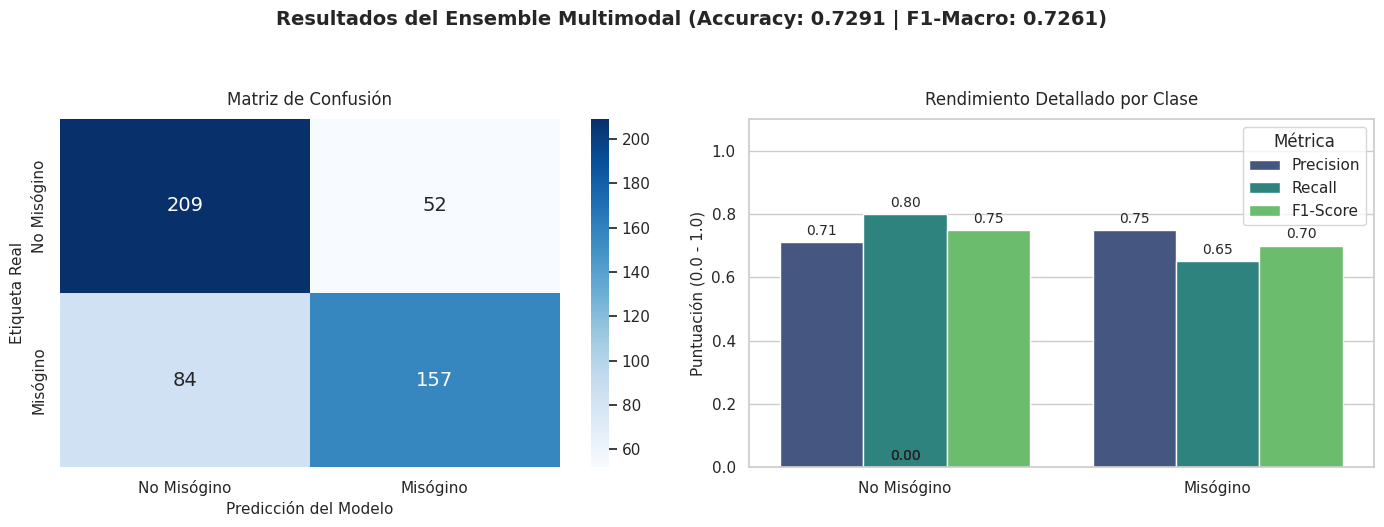
\includegraphics[width=0.9\textwidth]{Figuras/ResultadosEnsemble.png}
    \caption{Resultados del \textit{Ensemble} Multimodal contra el conjunto local de desarrollo}
    \label{fig:ResultadosEnsemble}
\end{figure}

\subsection{Análisis de Errores}
\label{subsec:AnalisisDeErrores}
Esta subsección tiene como objetivo detallar los errores cometidos por el sistema \textit{Ensemble} multimodal, buscando patrones o causas subyacentes que expliquen los fallos del modelo. No se trata únicamente de cuantificar las equivocaciones, sino de interpretarlas, comprendiendo en qué escenarios la inteligencia artificial encuentra dificultades para procesar la complejidad, el sarcasmo o la ambigüedad del lenguaje humano en las redes sociales. 

Sobre el conjunto local de desarrollo (502 instancias), el sistema generó un total de 136 predicciones erróneas. La contabilización de estas instancias en su matriz de confusión reveló un claro desbalance en el tipo de equivocación: 84 correspondieron a Falsos Negativos (el sistema no detectó el sexismo presente) y 52 a Falsos Positivos (el sistema generó una alarma falsa en un contenido inofensivo), acompañados de 209 Verdaderos Negativos y 157 Verdaderos Positivos. Esta distribución sugiere que el modelo adoptó una postura ligeramente conservadora, tendiendo a pasar por alto el sexismo cuando este se presenta de forma implícita o sutil. 

Es fundamental matizar que las explicaciones detalladas a continuación deben considerarse como interpretaciones razonables del comportamiento de la red neuronal. Al no haber implementado técnicas de Explicabilidad Algorítmica (\textit{XAI}) que muestren de forma empírica la atención de la red a características concretas, las causas atribuidas actúan como hipótesis derivadas de la observación. 

\subsubsection*{Identificación de errores comunes y ejemplos}
\label{subsubsec:IdentificacionDeErroresComunesYEjemplos}
Se estableció un protocolo de revisión cualitativa mediante el cual analizamos y codificamos manualmente una muestra de los 30 casos en los que el modelo mostró mayor ``confianza'' al equivocarse (es decir, aquellos donde la probabilidad arrojada estaba más alejada del umbral de decisión). Esto permitió agrupar los siguientes escenarios problemáticos:
\begin{itemize} 
    \item \underline{Ejemplo 1}: Violencia accidental confundida con violencia de género (Falso Positivo) 
    \begin{itemize} 
        \item \textbf{Texto}: ``\textit{cristiano ronaldo le regaló su camiseta a la guardia de seguridad que golpeó accidentalmente con un balonazo [...] la fuerza del pelotazo pues provocó que esta cayera al suelo por lo que tuvo inmediata atención...}''
        \item \textbf{Etiqueta real}: No sexista (0) | \textbf{Predicción}: Sexista (1)
        \item \textbf{Hipótesis}: Es altamente probable que el modelo asocie palabras clave de su vocabulario como ``golpeó'', ``cayera al suelo'' y ``mujer'' directamente con violencia física o machismo. Al carecer de la capacidad de abstracción para entender el contexto periodístico de un accidente deportivo, se dispara una falsa alarma.  
    \end{itemize}   
    \item \underline{Ejemplo 2}: Violencia digital contra grupos no objetivo de la tarea (Falso Positivo) 
    \begin{itemize} 
        \item \textbf{Texto}: ``\textit{el pibe inalcanzable que nunca dijo ni 'hola' en clase. se filtra su pack. compartan, compartan, muchachos, compartan...}''
        \item \textbf{Etiqueta real}: No sexista (0) | \textbf{Predicción}: Sexista (1)
        \item \textbf{Hipótesis}: El sistema detecta correctamente un patrón claro de un delito de violencia digital (difusión no consentida de imágenes íntimas mediante la palabra ``pack'' y la incitación a ``compartir''). Sin embargo, falla al razonar la directriz principal del reto: el sujeto pasivo de este escenario es un varón (el ``pibe''). Por consiguiente, aunque el texto describe un comportamiento tóxico, queda fuera de la definición estricta de discurso sexista o misógino contra la mujer que rige la construcción del \textit{dataset}, generando un falso positivo algorítmico.  
    \end{itemize} 
    \item \underline{Ejemplo 3}: \textit{Objectification} enmascarada y ruido de plataforma (Falso Negativo)
    \begin{itemize} 
        \item \textbf{Texto}: ``\textit{reply to stay smiling friends replying to yourmommaluvsthed's comment, i find chicks with jacked up teeth attractive. you must be in kentucky...}''
        \item \textbf{Etiqueta real}: Sexista (1) | \textbf{Predicción}: No sexista (0)
        \item \textbf{Hipótesis}: El mensaje contiene una clara cosificación y un uso despectivo hacia las mujeres (``\textit{chicks}''), pero el modelo no logró captar el sesgo implícito. Una posible explicación radica en que la ofensa es sutil, presentándose como una falsa preferencia estética. Además, la carga semántica está altamente diluida por los metadatos de la propia red social (``\textit{replying to... comment}''), una estructura sintáctica atípica de \textit{TikTok} que evadió los filtros de limpieza, lo que podría haber dificultado que el mecanismo de atención de la red se enfocase en la parte ofensiva.
    \end{itemize}
\end{itemize}

\subsubsection*{Errores por longitud y origen del texto}
\label{subsubsec:ErroresPorLongitudYOrigenDelTexto}
Al observar los errores en función de la estructura de las transcripciones, se registraron patrones descriptivos de interés. En primer lugar, la longitud media de los textos mal clasificados (91 palabras) resultó ser inferior a la media global del \textit{dataset} (103 palabras). Aunque sería necesario un análisis estadístico por intervalos para confirmar una correlación significativa, esta observación preliminar sugiere que los mensajes excesivamente cortos podrían privar a los modelos del contexto semántico necesario para entender la ironía o el sarcasmo, resultando en interpretaciones literales.

En segundo lugar, se identificó un desafío derivado de la diversidad en las fuentes del texto de entrada. La variable \texttt{text} proporcionada agrupa de forma indiferenciada texto proveniente de subtítulos superpuestos capturados por \textit{OCR}, transcripciones automáticas de voz (\textit{ASR}) e, incluso, metadatos y menciones a usuarios de la propia plataforma. Esta combinación produce transcripciones con nombres aleatorios y graves errores fonéticos o tipográficos. Planteamos la hipótesis de que esta densidad de ruido estructurado influye en la capacidad del modelo de aislar de manera precisa el verdadero discurso de odio del mensaje.

\subsubsection*{Reflexiones y posibles mejoras}
\label{subsubsec:ReflexionesYPosiblesMejoras}
El análisis cualitativo de estos fallos permite trazar líneas claras de trabajo a futuro. Una posible mejora radicaría en la aplicación de un preprocesamiento mucho más avanzado sobre el corpus, incorporando modelos de corrección ortográfica e identificadores de entidades nombradas para purgar nombres de usuario y menciones atípicas. 

Asimismo, se podrían generar más ejemplos de sexismo benevolente, humor sarcástico e incidentes violentos no relacionados con el género, para que el sistema aprenda a definir las fronteras o límites del sexismo. Finalmente, el uso de modelos auxiliares previamente entrenados en la detección exclusiva de ironía podría añadirse al \textit{Ensemble} como una característica de entrada adicional, ayudando a mitigar la alta tasa de Falsos Negativos detectada.

A modo de conclusión general, la optimización del sistema \textit{Ensemble} indica un buen ajuste a este complejo contenido, alcanzando un pico de \textit{Accuracy} local de 0.7291 y un \textit{F1-score} de 0.7261. Reiteramos que es fundamental interpretar este valor de 0.7261 como una métrica de calibración interna ajustada al conjunto exploratorio.  

De hecho, un análisis profundo revela sesgos predictivos importantes inherentes a esta calibración. Si observamos el rendimiento detallado por clase (apoyado en la matriz de TN=209, FP=52, FN=84 y TP=157), el modelo muestra un comportamiento notoriamente conservador: es más robusto al identificar instancias inofensivas (\textit{Recall} de 0.80 para la clase No Sexista) que al detectar agresiones reales (\textit{Recall} de 0.65 para la clase Sexista). 

Esta diferencia de 15 puntos porcentuales es la causa directa de la acumulación de Falsos Negativos. En la práctica, el ajuste del sistema priorizó no penalizar a usuarios inocentes (manteniendo bajos los Falsos Positivos), a costa de permitir que discursos de odio sutiles o enmascarados bajo ironía eludan el filtro. 

\subsection{Evaluación Final sobre el Conjunto de \textit{Test Ciego}}
\label{subsec:EvaluacionFinalTestCiego}
Tras la calibración interna del sistema explicada en las secciones anteriores, se procedió a la fase de evaluación definitiva. Con el objetivo de validar verdaderamente el modelo, se ejecutó la inferencia completa sobre el conjunto de \textit{Test} ciego oficial proporcionado por la organización del reto \textit{EXIST 2025} (compuesto por 674 vídeos sin etiquetar), el cual garantiza la separación rigurosa de autores para evitar fuga de información.

Las predicciones binarias generadas por el \textit{Ensemble} fueron enviadas a la plataforma oficial de evaluación del reto \footnote{\url{https://evall.uned.es/}}. En la \autoref{tab:ResultadosOficialesEnsemble} se presentan las métricas finales emitidas por el sistema \textit{PyEvALL}.

\begin{table}[H]
    \centering
    \begin{tabular}{lcccc}
        \toprule
        \textbf{Envío Oficial} & 
        \textbf{\begin{tabular}[c]{@{}c@{}}Ranking \\ Hipotético\end{tabular}} & 
        \textbf{ICM-Hard} & 
        \textbf{\begin{tabular}[c]{@{}c@{}}ICM-Hard \\ Norm\end{tabular}} & 
        \textbf{F1 Macro} \\
        \midrule
        \begin{tabular}[c]{@{}l@{}}\textit{Ensemble Multimodal} \\ (\textit{Late Fusion})\end{tabular} & 34 & -0.1008 & 0.4491 & 0.6311 \\
        \bottomrule
    \end{tabular}
    \caption{Resultados oficiales obtenidos en la Subtarea 3.1 de \textit{EXIST 2025} con el modelo \textit{Ensemble}}
    \label{tab:ResultadosOficialesEnsemble}
\end{table}

Al contrastar esta evaluación independiente con las métricas de las entregas unimodales iniciales del reto (detalladas previamente en la \autoref{tab:ResultadosOficialesEXIST}), se observa una mejora en el rendimiento del sistema. El \textit{Ensemble} alcanza un \textit{ICM Norm} de 0.4491, superando el 0.4355 de nuestro mejor envío oficial (\textit{BERT}) y distanciándose significativamente del 0.2874 obtenido por el modelo generativo \textit{LLaMA}.

Como es habitual en este tipo de investigaciones, se registra una caída en el rendimiento al pasar del entorno de selección local (\textit{F1}: 0.7261) al entorno ciego (\textit{F1}: 0.6311), evidenciando el \textit{overfitting} del conjunto exploratorio reutilizado y la dificultad que presentan las nuevas distribuciones de datos. Sin embargo, la evolución positiva respecto a los \textit{baselines} oficiales sugiere que la estrategia de fusión multimodal aporta una mayor robustez frente al problema. La combinación del análisis espacial de la imagen con la transcripción textual resulta de gran utilidad para contextualizar el mensaje, mitigando parte de la ambigüedad presente en las redes sociales y estableciendo una base más sólida para la moderación automática. 

\section{Perspectivismo en \textit{LeWiDi}}
\label{sec:PerspectivismoEnLewidi}
El reto \textit{EXIST 2025} introduce un desafío pionero en el campo de la detección del sexismo: la noción de que el sexismo, especialmente en sus formas más sutiles (como micromachismos y paternalismos), no siempre goza de un consenso absoluto. La percepción de si un comentario es sexista o inofensivo puede variar significativamente dependiendo de los sesgos culturales, las vivencias personales y, particularmente, el género del individuo que lo evalúa. Esta pluralidad de visiones se fundamenta teóricamente en el \textbf{Perspectivismo}, un concepto que reconoce la subjetividad en la interpretación del discurso. En el ámbito del aprendizaje automático, esta noción se materializa a través del paradigma \textbf{\textit{Learning with Disagreement} (\textit{LeWiDi})}, el cual defiende que el desacuerdo empírico entre anotadores no es un ``ruido'' estadístico que deba limpiarse, sino una señal rica en información que debe modelarse.

En las secciones anteriores, los modelos se entrenaron mediante ``Consenso Mayoritario'' (fusionando todas las opiniones en una sola etiqueta unificada). En esta última fase experimental referente a la Tarea 3.1, se buscará explorar cómo varía el rendimiento empírico de las redes neuronales cuando se filtran los datos de entrenamiento por el género del anotador o se instruye a un modelo generativo a simular un rol. 

\subsection{Segmentación demográfica en \textit{Transformers}}
\label{subsec:SegmentacionDemograficaEnTransformers}
La primera aproximación al perspectivismo consistió en entrenar modelos discriminativos independientes basados en los datos demográficos de los anotadores humanos. A partir del conjunto de entrenamiento maestro, se extrajeron de forma aislada los votos emitidos exclusivamente por los anotadores masculinos y, en paralelo, los emitidos por las anotadoras femeninas. 

Dado que un mismo vídeo podía ser evaluado por varios anotadores del mismo género (por ejemplo, dos hombres), surgieron casos de empate o ``disidencia interna'' (un hombre etiquetando como 1 y otro como 0). Para abordar este desacuerdo interno de manera metodológica y utilizando la arquitectura \texttt{RoBERTa-base}, se entrenaron 8 conjuntos de datos distintos (4 estrategias x 2 géneros): 
\begin{itemize}
    \item \textbf{Descartes (\textit{Hard Consensus})}: Se eliminaron del entrenamiento aquellos vídeos en los que los anotadores humanos del mismo género no lograron ponerse de acuerdo. 
    \item \textbf{Ante la duda, Sexismo (\textit{Pessimistic})}: En caso de empate interno humano, el video se etiquetó como sexista (1).
    \item \textbf{Ante la duda, No Sexismo (\textit{Optimistic})}: En caso de empate interno humano, prevaleció la presunción de inocencia y se etiquetó como no sexista (0).
    \item \textbf{Desenrollado (\textit{Unrolling})}: No se forzó ningún consenso. Si un vídeo presentaba empate, se introdujo dos veces en el dataset: una fila con etiqueta 1 y otra fila idéntica con etiqueta 0, obligando al modelo a asimilar la dualidad de la anotación.
\end{itemize}

Para interpretar de forma científica los resultados de esta fase, es fundamental analizar la distribución resultante tras aplicar estas estrategias. En la \autoref{tab:DistribucionPerspectivismo} se exponen los tamaños y el balance de clases de cada subconjunto de datos.

\begin{table}[H]
    \centering
    \begin{tabular}{llccc}
    \toprule
    \textbf{Estrategia} & \textbf{Género} & \textbf{Total Vídeos} & \textbf{No Sexista (0)} & \textbf{Sexista (1)} \\
    \midrule
    \multirow{2}{*}{Descartes} & Femenino & 1984 & 1035 & 949 \\
    & Masculino & 1396 & 787 & 609 \\
    \midrule
    \multirow{2}{*}{\textit{Pessimistic}} & Femenino & 2006 & 1035 & 971 \\
    & Masculino & 1612 & 787 & 825 \\
    \midrule
    \multirow{2}{*}{\textit{Optimistic}} & Femenino & 2006 & 1057 & 949 \\
    & Masculino & 1612 & 1003 & 609 \\
    \midrule
    \multirow{2}{*}{\textit{Unrolling}} & Femenino & 2644 & 1372 & 1272 \\
    & Masculino & 1948 & 1056 & 892 \\
    \bottomrule
    \end{tabular}
    \caption{Distribución de los \textit{datasets} de entrenamiento tras la segmentación por género y aplicación de estrategias de resolución de empates.}
    \label{tab:DistribucionPerspectivismo}
\end{table}

Debe reconocerse una limitación a la hora de comparar estos modelos frente al conjunto local de desarrollo (\textit{Gold Standard} unificado de 502 instancias). Como se evidencia en la tabla, existe un factor: los \textit{datasets} basados en anotaciones femeninas poseen un mayor volumen de datos que los masculinos. Por tanto, las variaciones en el rendimiento no pueden atribuirse exclusivamente a diferencias intrínsecas en la perspectiva de género, sino que podrían estar directamente influenciadas por la diferencia en la cantidad de ejemplos expuestos a la red durante el entrenamiento.

\begin{figure}[H]
    \centering
    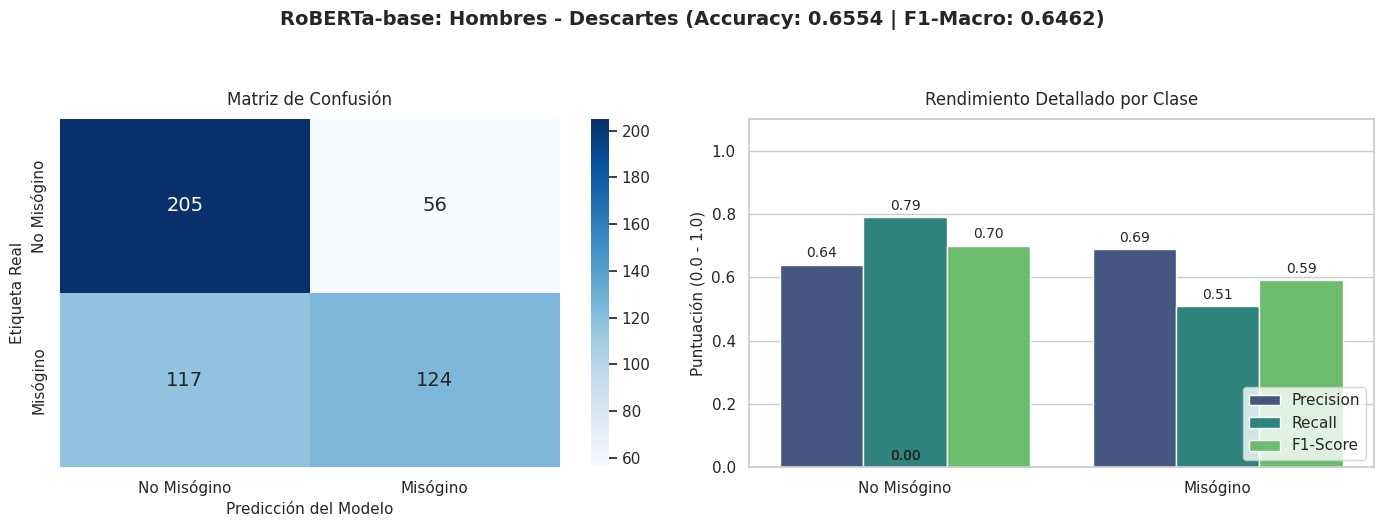
\includegraphics[width=0.9\textwidth]{Figuras/ResultadosHombreDiscard.png}
    \caption{Resultados de la estrategia \textit{Hard Consensus} en hombres}
    \label{fig:ResultadosTransformersPerspectivismoHombreDiscard}
\end{figure}
\begin{figure}[H]
    \centering
    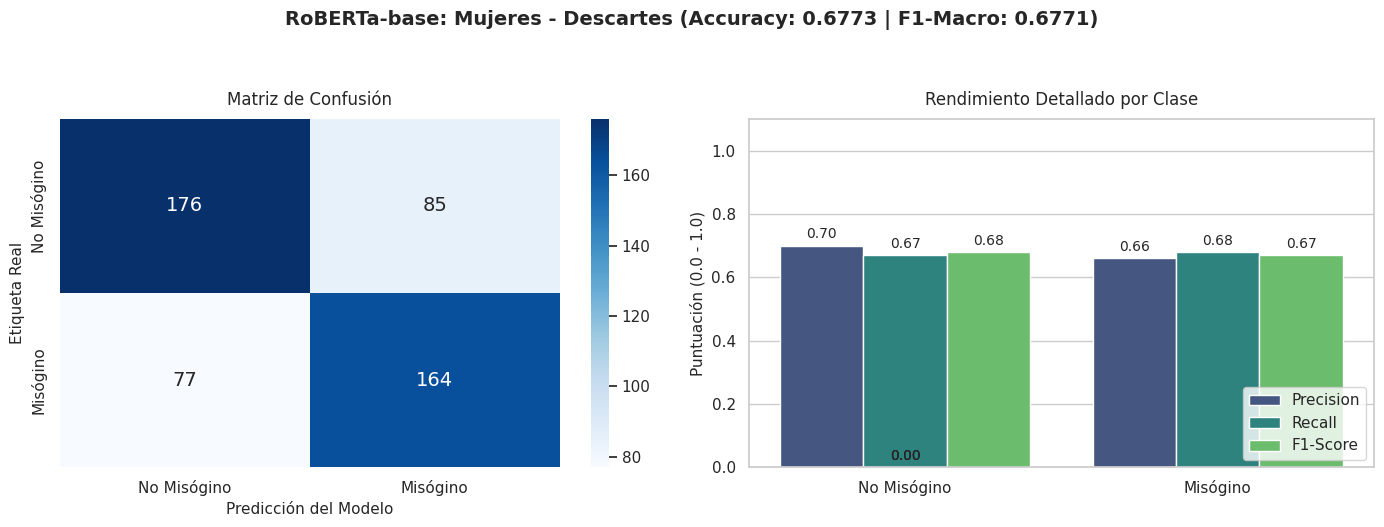
\includegraphics[width=0.9\textwidth]{Figuras/ResultadosMujerDiscard.png}
    \caption{Resultados de la estrategia \textit{Hard Consensus} en mujeres}
    \label{fig:ResultadosTransformersPerspectivismoMujerDiscard}
\end{figure}

En la \autoref{fig:ResultadosTransformersPerspectivismoHombreDiscard} y en la \autoref{fig:ResultadosTransformersPerspectivismoMujerDiscard}, se evaluó el rendimiento tras aplicar la estrategia de Descartes:
\begin{itemize}
    \item \textbf{Perspectiva Femenina}: El modelo entrenado con estos datos logra un \textit{F1-score} de 0.6771. Según se observa en su respectiva matriz de confusión, identifica 164 Verdaderos Positivos frente a los 124 del modelo masculino, alcanzando un \textit{Recall} de 0.68 para la clase sexista.
    \item \textbf{Perspectiva Masculina}: Presenta un \textit{F1-score} de 0.6462. Como evidencia su matriz, su \textit{Recall} para la clase sexista decae a 0.51, registrando 117 Falsos Negativos frente a 124 Verdaderos Positivos sobre el conjunto de validación unificado.
\end{itemize}

\begin{figure}[H]
    \centering
    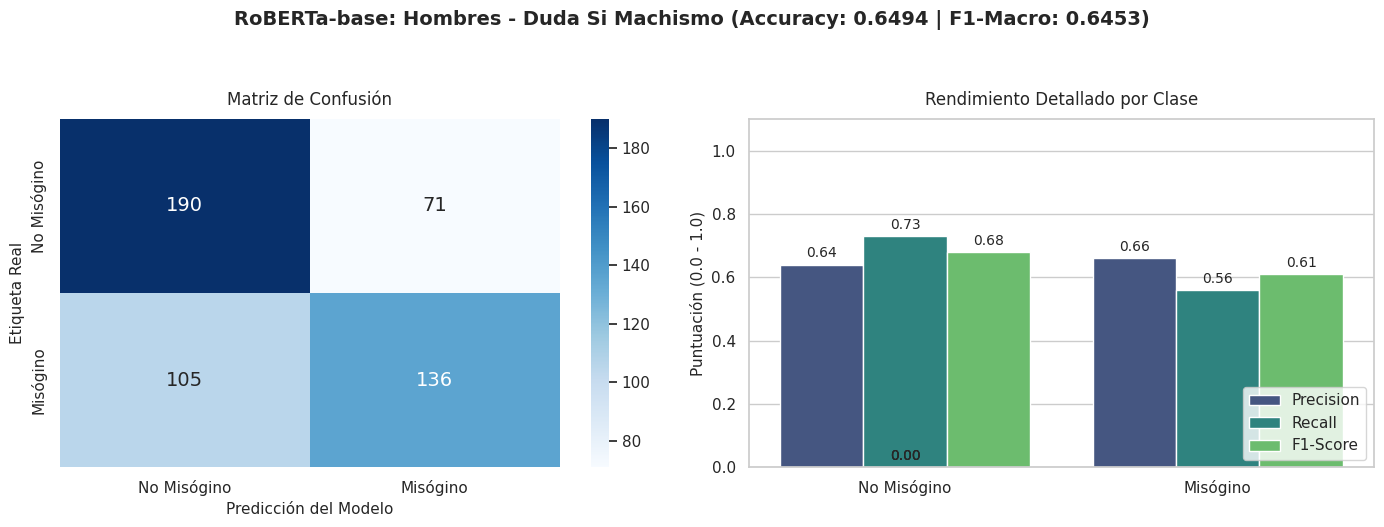
\includegraphics[width=0.9\textwidth]{Figuras/ResultadosHombrePessimistic.png}
    \caption{Resultados de la estrategia \textit{Pessimistic} en hombres}
    \label{fig:ResultadosTransformersPerspectivismoHombrePessimistic}
\end{figure}
\begin{figure}[H]
    \centering
    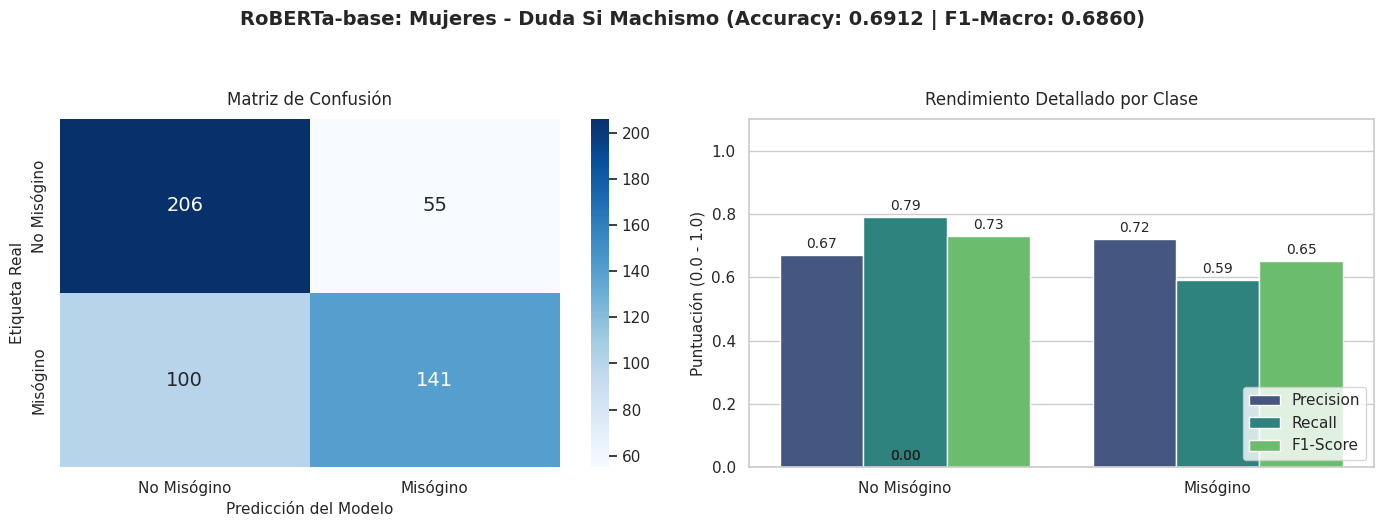
\includegraphics[width=0.9\textwidth]{Figuras/ResultadosMujerPessimistic.png}
    \caption{Resultados de la estrategia \textit{Pessimistic} en mujeres}
    \label{fig:ResultadosTransformersPerspectivismoMujerPessimistic}
\end{figure}

En la \autoref{fig:ResultadosTransformersPerspectivismoHombrePessimistic} y en la \autoref{fig:ResultadosTransformersPerspectivismoMujerPessimistic}, asumiendo la etiqueta sexista en caso de empate humano, las métricas muestran el siguiente comportamiento:
\begin{itemize}
    \item \textbf{Perspectiva Femenina}: Alcanza aquí el mejor rendimiento global registrado en esta fase (\textit{F1-score} de 0.6860). La adopción de esta postura conservadora no dispara de forma descontrolada los Falsos Positivos, conservando una \textit{Precisión} de 0.72 para la clase positiva.
    \item \textbf{Perspectiva Masculina}: El modelo disminuye su rendimiento bajo esta directriz (F1: 0.6453). Al obligarle a asumir la etiqueta sexista en los empates, el modelo incrementa los errores al clasificar instancias de la clase 0.
\end{itemize}

\begin{figure}[H]
    \centering
    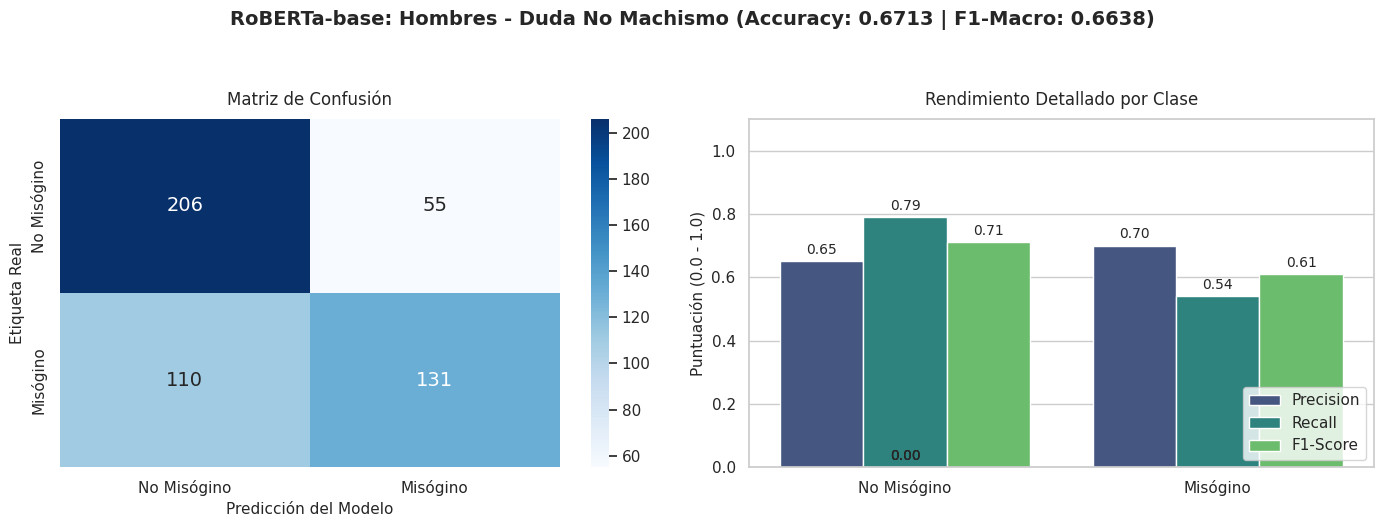
\includegraphics[width=0.9\textwidth]{Figuras/ResultadosHombreOptimistic.png}
    \caption{Resultados de la estrategia \textit{Optimistic} en hombres}
    \label{fig:ResultadosTransformersPerspectivismoHombreOptimistic}
\end{figure}
\begin{figure}[H]
    \centering
    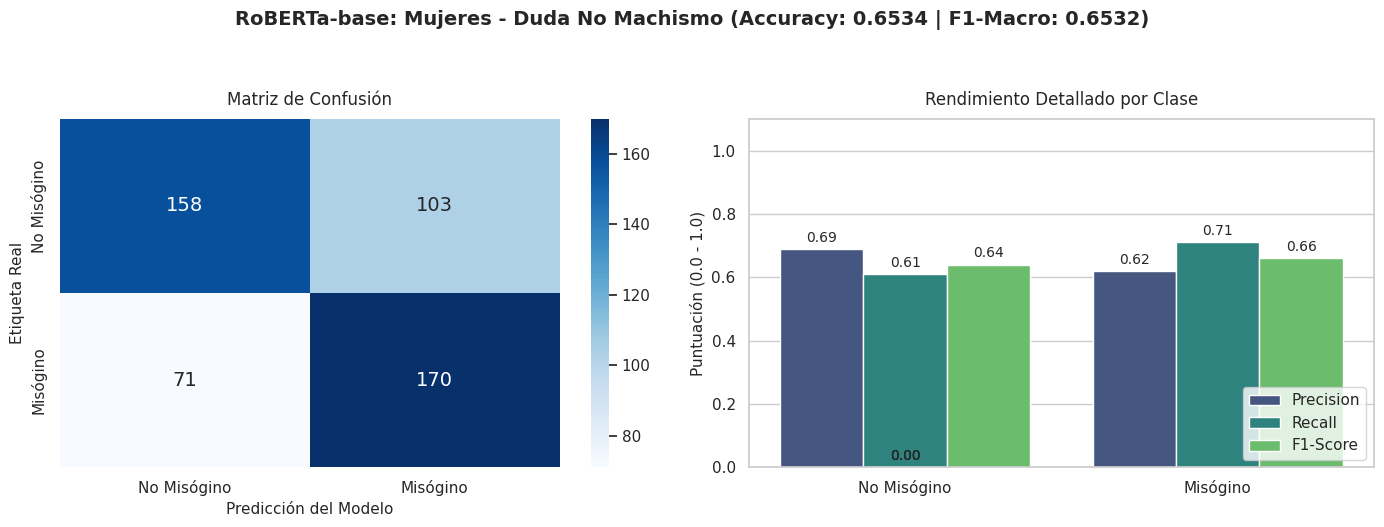
\includegraphics[width=0.9\textwidth]{Figuras/ResultadosMujerOptimistic.png}
    \caption{Resultados de la estrategia \textit{Optimistic} en mujeres}
    \label{fig:ResultadosTransformersPerspectivismoMujerOptimistic}
\end{figure}

En la \autoref{fig:ResultadosTransformersPerspectivismoHombreOptimistic} y en la \autoref{fig:ResultadosTransformersPerspectivismoMujerOptimistic}, asumiendo la etiqueta no sexista en los empates, se observa:
\begin{itemize}
    \item \textbf{Perspectiva Masculina}: El modelo presenta un \textit{Recall} de 0.54 para la clase sexista, arrojando 110 Falsos Negativos en su matriz frente a los datos del \textit{Gold Standard}.
    \item \textbf{Perspectiva Femenina}: Su \textit{Recall} para la clase sexista se sitúa en 0.71, reduciendo los Falsos Negativos a 71.
\end{itemize}

\begin{figure}[H]
    \centering
    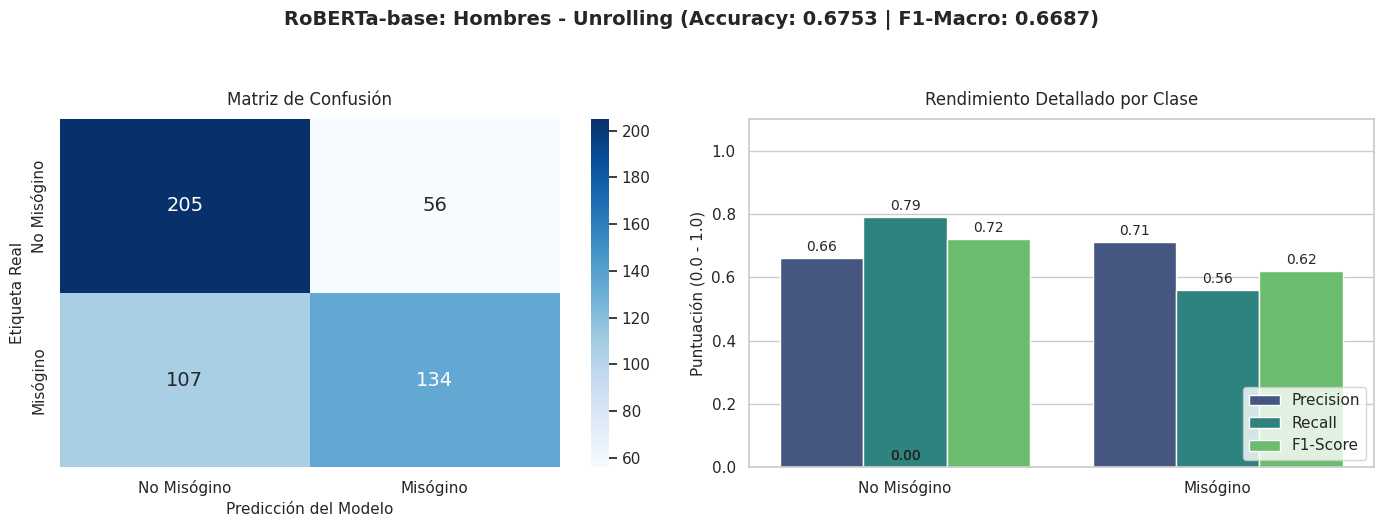
\includegraphics[width=0.9\textwidth]{Figuras/ResultadosHombreUnrolling.png}
    \caption{Resultados de la estrategia \textit{Unrolling} en hombres}
    \label{fig:ResultadosTransformersPerspectivismoHombreUnrolling}
\end{figure}
\begin{figure}[H]
    \centering
    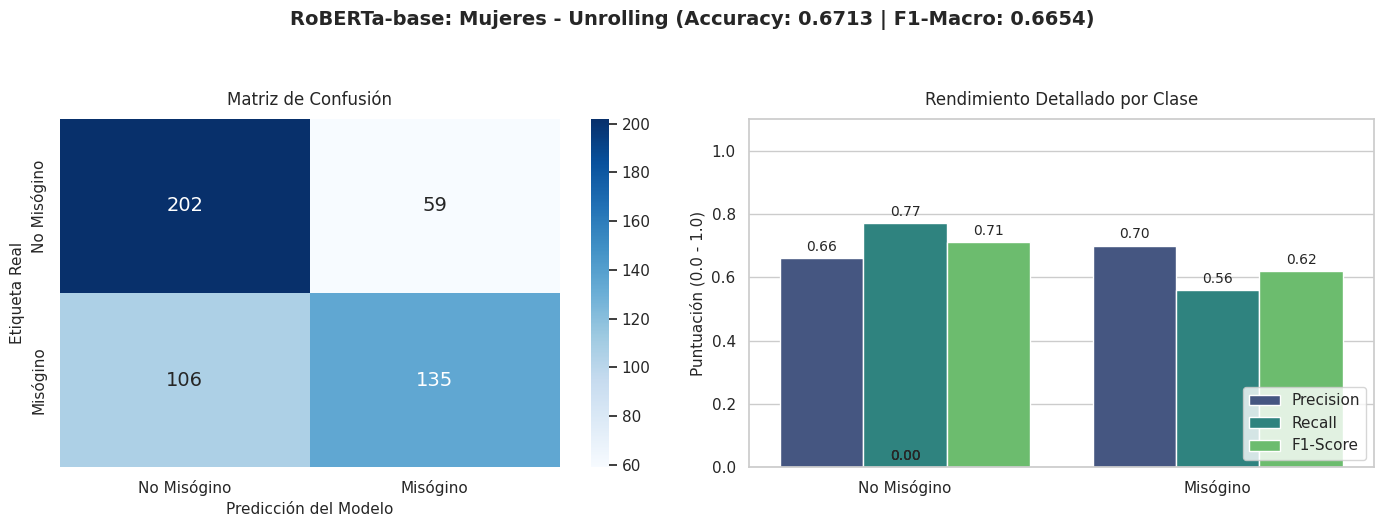
\includegraphics[width=0.9\textwidth]{Figuras/ResultadosMujerUnrolling.png}
    \caption{Resultados de la estrategia \textit{Unrolling} en mujeres}
    \label{fig:ResultadosTransformersPerspectivismoMujerUnrolling}
\end{figure}

Como podemos observar en la \autoref{fig:ResultadosTransformersPerspectivismoHombreUnrolling} y en la \autoref{fig:ResultadosTransformersPerspectivismoMujerUnrolling}, la aplicación de \textit{Unrolling} produce un ajuste evidente en ambos perfiles: 
\begin{itemize}
    \item \textbf{Convergencia de métricas}: Al duplicar los datos empatados, las diferencias de rendimiento entre el conjunto de entrenamiento de hombres (\textit{F1-score}: 0.6687) y el de mujeres (\textit{F1-score}: 0.6654) prácticamente desaparecen.
    \item \textbf{Análisis}: Ambos modelos calcan sus métricas de \textit{Recall} para la clase Sexista (0.56). Esta similitud sugiere que la estrategia de desenrollado, al exponer a la red a la dualidad de las etiquetas, homogeneiza el comportamiento predictivo, difuminando el impacto del filtrado demográfico original.
\end{itemize}

\subsection{Análisis de Sensibilidad al \textit{Prompt} en \textit{LLMs} (\textit{Persona Prompting})}
\label{subsec:InyeccionDeRolesEnLLMs}
La segunda estrategia evaluó la sensibilidad de los modelos generativos ante variaciones semánticas en la instrucción (\textit{Prompt Engineering}). Es esencial clarificar que el objetivo de este experimento no es simular de forma válida perspectivas humanas reales, sino cuantificar cómo la alteración explícita de la palabra clave asociada al género en el \textit{prompt} activa diferentes sesgos estadísticos preadquiridos por la inteligencia artificial.

Aprovechando la capacidad de los \textit{LLMs} para adaptar sus salidas, se aplicó la técnica de \textit{Persona Prompting} sobre el modelo \texttt{Mistral-7B-Instruct-v0.3} en un entorno \textit{Zero-Shot}. En lugar de pedirle una clasificación neutral, se diseñaron dos \textit{prompts} que inyectaron una instrucción de rol directamente en el contexto del modelo. El \textit{prompt} diseñado fue el siguiente:

\begin{tcolorbox}[colback=gray!10, colframe=gray!40, arc=4pt, boxrule=0.5pt]
    \texttt{[INST]} Actúa como un hombre. Eres un experto analizando redes sociales. Clasifica el siguiente texto en una de estas dos categorías: 'Sexista' o 'No Sexista'. Devuelve ÚNICAMENTE la etiqueta correspondiente, sin explicaciones adicionales. Texto: \{texto\} \texttt{[/INST]} 
    Etiqueta:
\end{tcolorbox}

De manera simétrica, para evaluar la instrucción opuesta, se sustituyeron exclusivamente las referencias de género (``Actúa como una mujer'', ``Eres una experta...'').

En las \autoref{fig:ResultadosPromptHombre} y \autoref{fig:ResultadosPromptMujer} se puede observar cómo la inyección del rol altera la distribución de las predicciones del modelo frente a los mismos 502 registros del \textit{Test} de desarrollo.

\begin{figure}[H]
    \centering
    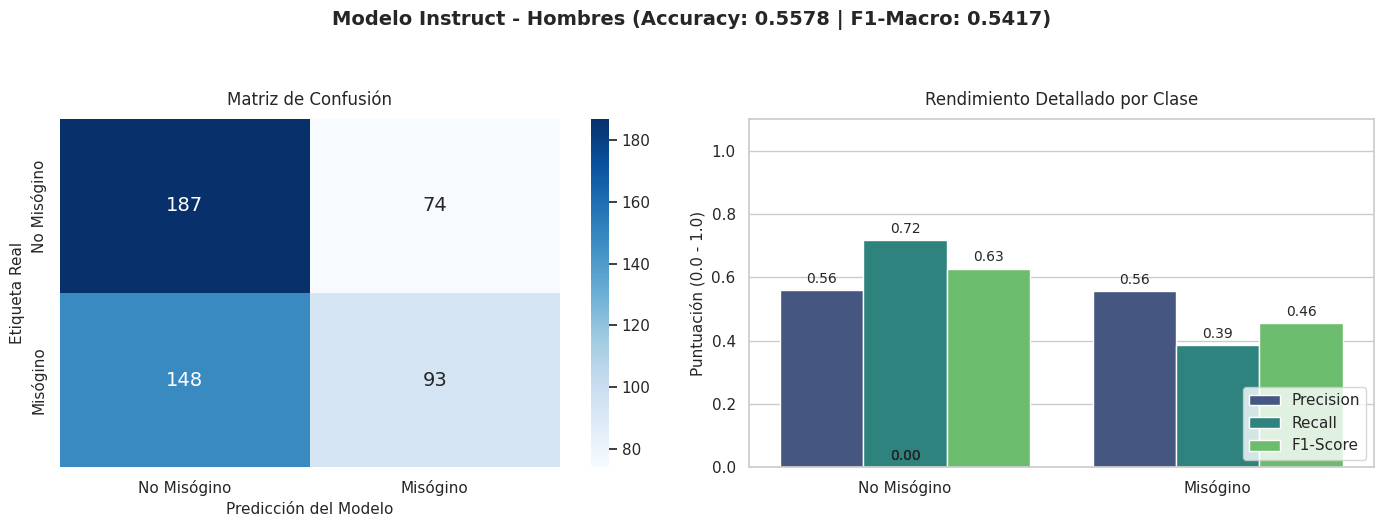
\includegraphics[width=0.9\textwidth]{Figuras/ResultadosPromptHombre.png}
    \caption{Resultados de la técnica \textit{Persona Prompting} instruyendo el rol de hombre}
    \label{fig:ResultadosPromptHombre}
\end{figure}
\begin{figure}[H]
    \centering
    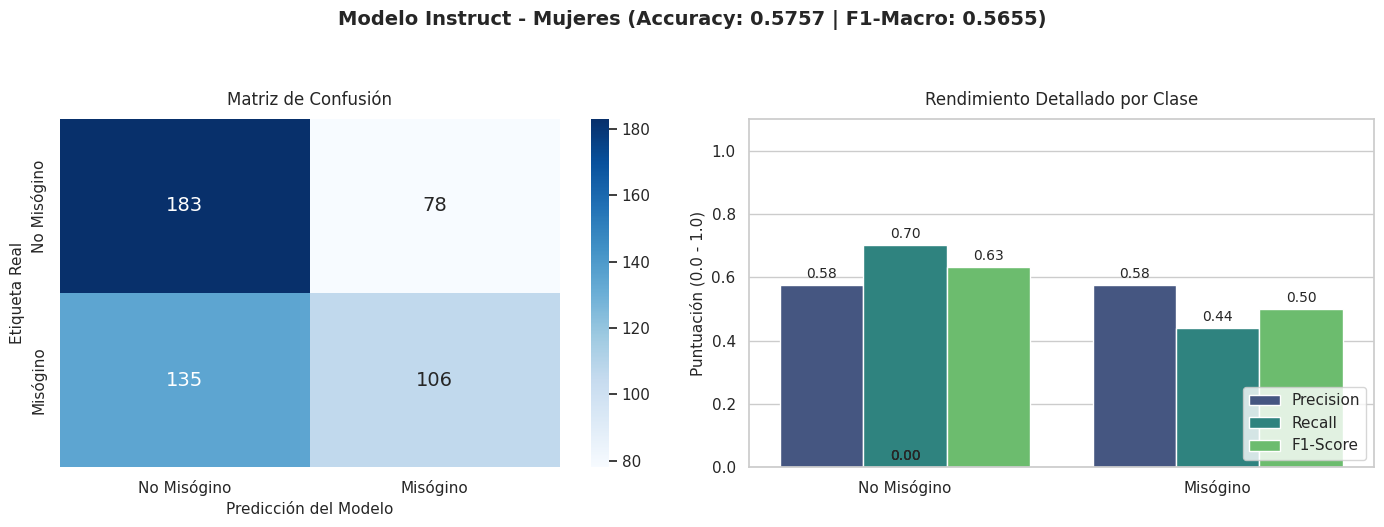
\includegraphics[width=0.9\textwidth]{Figuras/ResultadosPromptMujer.png}
    \caption{Resultados de la técnica \textit{Persona Prompting} instruyendo el rol de mujer}
    \label{fig:ResultadosPromptMujer}
\end{figure}

\subsection{Análisis de los Resultados Exploratorios}
\label{subsec:AnalisisDeLosResultadosDePerspectivismo}
Para facilitar la comparativa de los impactos demográficos detallados en las secciones anteriores, en la \autoref{tab:ResumenPerspectivismo} se aglutinan los resultados obtenidos por todas las arquitecturas y estrategias tras la segmentación por género.

\begin{table}[H]
    \centering
    \begin{tabular}{llccc}
    \toprule
    \textbf{Arquitectura} & \begin{tabular}[c]{@{}l@{}}\textbf{Estrategia de} \\ \textbf{\textit{LeWiDi}}\end{tabular} & \textbf{Rol / Género} & \textbf{\textit{Accuracy}} & \begin{tabular}[c]{@{}c@{}}\textbf{\textit{F1-score}} \\ \textbf{(Macro)}\end{tabular} \\
    \midrule
    \multirow{8}{*}{\texttt{RoBERTa-base}} 
        & \multirow{2}{*}{\begin{tabular}[c]{@{}l@{}}Descartes \\ (\textit{Hard Consensus})\end{tabular}} 
            & Femenino & 0.6773 & 0.6771 \\
        & & Masculino & 0.6554 & 0.6462 \\
    \addlinespace[0.5em]
        & \multirow{2}{*}{\begin{tabular}[c]{@{}l@{}}\textit{Pessimistic} \\ (Duda = Sexismo)\end{tabular}} 
            & Femenino & 0.6912 & 0.6860 \\
        & & Masculino & 0.6494 & 0.6453 \\
    \addlinespace[0.5em]
        & \multirow{2}{*}{\begin{tabular}[c]{@{}l@{}}\textit{Optimistic} \\ (Duda = Inocencia)\end{tabular}} 
            & Femenino & 0.6534 & 0.6532 \\
        & & Masculino & 0.6713 & 0.6638 \\
    \addlinespace[0.5em]
        & \multirow{2}{*}{\begin{tabular}[c]{@{}l@{}}Desenrollado \\ (\textit{Unrolling})\end{tabular}} 
            & Femenino & 0.6713 & 0.6654 \\
        & & Masculino & 0.6753 & 0.6687 \\
    \midrule
    \multirow{2}{*}{\texttt{Mistral-7B-Instruct}} 
        & \multirow{2}{*}{\begin{tabular}[c]{@{}l@{}}\textit{Persona} \\ \textit{Prompting}\end{tabular}} 
            & \begin{tabular}[c]{@{}l@{}}Instrucción \\ Femenina\end{tabular} & 0.5757 & 0.5655 \\
        & & \begin{tabular}[c]{@{}l@{}}Instrucción \\ Masculina\end{tabular} & 0.5578 & 0.5417 \\
    \bottomrule
    \end{tabular}
    \caption{Rendimiento comparativo de las estrategias exploratorias filtradas por género.}
    \label{tab:ResumenPerspectivismo}
\end{table}

El análisis de estos resultados permite extraer varias observaciones descriptivas sobre el comportamiento de las redes neuronales en este escenario. En primer lugar, los modelos \textit{Transformers} entrenados con los \textit{datasets} femeninos alcanzaron de forma consistente métricas más altas frente al \textit{Gold Standard} unificado (pico de \textit{F1-score} de 0.6860) que sus contrapartes masculinas (cuyo máximo se situó en 0.6687). No obstante, como se advirtió previamente, el riesgo de un sesgo por el tamaño de la muestra impide concluir con seguridad que existan características superiores en dichas anotaciones.
 
En segundo lugar, se observan diferencias ante la gestión empírica de la duda. Mientras que la variante \textit{Pessimistic} maximizó el rendimiento en el \textit{dataset} filtrado femenino, en el caso del masculino la mejor respuesta se obtuvo preservando la ambigüedad mediante \textit{Unrolling}.

Finalmente, los resultados de \textit{Persona Prompting} evidencian la adaptación de los \textit{LLMs} a los sesgos inducidos por la formulación de la instrucción. El modelo instruido con la palabra ``mujer'' logró un \textit{F1-score} de 0.5655, frente al 0.5417 arrojado bajo la instrucción ``hombre''. Al examinar sus matrices, el \textit{prompt} masculino generó una tasa mayor de Falsos Negativos (148 instancias frente a las 135 generadas por el \textit{prompt} femenino). Planteamos como hipótesis que la inyección de la palabra ``hombre'' activa estereotipos estadísticos preentrenados en la red que  derivan en una evaluación más restrictiva a la hora de tipificar el sexismo.

Es importante remarcar que el diseño metodológico de toda esta fase es de naturaleza exploratoria. Las métricas exponen el comportamiento de los modelos y las variaciones de los \textit{datasets}, y en ningún caso deben extrapolarse para formular juicios psicológicos o sociológicos sobre el comportamiento real de hombres y mujeres.

\section{Experimentación Multietiqueta (Tarea 3.3)}
\label{sec:ExperimentacionMultietiqueta}
La Tarea 3.3 del desafío \textit{EXIST 2025} plantea un problema de clasificación mucho más específico y complejo que la mera detección binaria, estructurándose como un reto jerárquico y multietiqueta. En su formulación original, el sistema debe primero discriminar si un contenido es sexista o inofensivo (primer nivel de la jerarquía) y, únicamente en caso afirmativo, categorizarlo en una o varias de cinco tipologías concretas simultáneamente (clasificación multietiqueta en el segundo nivel).

Cabe matizar explícitamente que la experimentación detallada en esta sección constituye un análisis parcial y exploratorio de las capacidades de los modelos para fines puramente académicos, por lo que no reproduce la evaluación jerárquica completa de la subtarea 3.3 oficial de \textit{EXIST 2025}. Para acotar el alcance de este Trabajo de Fin de Máster, se ha definido un análisis condicionado: se asume que el primer nivel jerárquico ya está resuelto, filtrando el conjunto de datos para evaluar a los modelos exclusivamente sobre los vídeos que ya estaban catalogados previamente como sexistas.

Asimismo, en lugar de desplegar una única arquitectura compleja con una capa de salida multietiqueta conjunta, el problema se ha abordado de forma simplificada mediante una estrategia conocida como \textit{Binary Relevance} o \textit{One-vs-Rest}. Se ha aislado cada categoría y se han entrenado clasificadores binarios independientes para cada tipología. Si bien esto simplifica la fase de optimización, conlleva una limitación estructural: las redes no son capaces de aprender las posibles correlaciones entre las distintas categorías de sexismo.

Bajo este entorno controlado, las cinco categorías evaluadas son:
\begin{itemize}
    \item \textbf{\textit{Ideological and Inequality}}: El texto desacredita el movimiento feminista, rechaza la desigualdad de género o victimiza a un hombre. 
    \item \textbf{\textit{Stereotyping and Dominance}}: Expresa ideas falsas sobre los roles de la mujer (sumisa o cuidadora) o tareas inadecuadas, afirmando la superioridad masculina. 
    \item \textbf{\textit{Objectification}}: Presenta a la mujer como un objeto, describiendo cualidades físicas obligatorias para cumplir cánones de belleza o hipersexualización.
    \item \textbf{\textit{Sexual Violence}}: Sugerencias sexuales, petición de favores o acoso explícito de naturaleza sexual (violación o agresión).
    \item \textbf{\textit{Misogyny and Non-Sexual Violence}}: Expresión de odio puro y violencia no sexual hacia las mujeres. 
\end{itemize}

Para abordar esta tarea, se replicó la metodología de experimentación unimodal utilizada en la Tarea 3.1. Se seleccionó el modelo con mejor rendimiento de cada familia arquitectónica para entrenarlo de manera independiente frente a cada una de las 5 etiquetas:
\begin{itemize}
    \item \textbf{\textit{Transformers}}: \texttt{roberta-base}.
    \item \textbf{\textit{LLM}}: \texttt{Mistral-7B-Instruct}. 
    \item \textbf{Visión Estática}: \texttt{ConvNeXt}, entrenado sobre secuencias de 4 \textit{frames}.
    \item \textbf{Visión Temporal}: \texttt{TimeSFormer}, procesando 16 \textit{frames} por inferencia.
\end{itemize}

\subsection{Preparación del Dataset Multietiqueta}
\label{subsec:PreparacionDelDatasetMultietiqueta}
A diferencia de la Tarea 3.1, la naturaleza multietiqueta del problema requiere un tratamiento especial de los datos. A partir del \textit{JSON} original, se filtraron exclusivamente aquellos vídeos catalogados previamente como sexistas (etiqueta 1 en la Tarea 3.1). Para unificar las discrepancias entre anotadores respecto al tipo de sexismo detectado, se aplicó una lógica \textit{OR}: si al menos un anotador marcaba una de las cinco etiquetas en su evaluación, el vídeo se consideraba positivo para dicha clase. 

Es necesario reconocer que esta heurística de unificación transforma la incertidumbre del \textit{Learning with Disagreement} (\textit{LeWiDi}) en etiquetas rígidas (\textit{Hard Labels}), perdiendo la distribución suave original y tendiendo a sobre-representar las categorías (sesgo hacia la sensibilidad). Por tanto, estas etiquetas actúan como un terreno de calibración experimental y no deben interpretarse como una verdad absoluta y neutral.

Dado el fuerte desbalance intrínseco en la distribución de las subcategorías, la división del conjunto original en \textit{Train} (80\%) y \textit{Test} (20\%) se ejecutó mediante la función \texttt{iterative\_train\_test\_split} de la librería \texttt{skmultilearn}. Este enfoque garantiza un particionado estratificado, asegurando que las proporciones de las clases minoritarias se mantengan estables en ambos subconjuntos. A partir de este \textit{CSV} maestro, se generaron las réplicas correspondientes para el entrenamiento de visión estática y temporal. 

\subsection{Resultados y Análisis Cruzado por Tipología}
\label{subsec:ResultadosYAnalisisCruzadoPorTipologia}
El entrenamiento aislado de los cuatro mejores modelos contra las cinco etiquetas reveló un comportamiento dependiente de la modalidad de los datos (texto frente a imagen/movimiento) y de la distribución estadística de cada clase. En la \autoref{tab:ResultadosEntrenamientosMultietiqueta} se resumen las métricas \textit{F1-Score (Macro)} y \textit{Accuracy} obtenidas sobre el conjunto de \textit{Test} de desarrollo multietiqueta. Dado el enfoque de \textit{Binary Relevance}, las métricas se reportan de forma aislada por etiqueta y no se incluyen métricas globales \textit{multilabel}.

\begin{table}[H]
    \centering
    \begin{tabular}{lllcc}
        \toprule
        \textbf{Etiqueta} & \textbf{Modelo} & \textbf{Inferencia} & \textbf{Accuracy} & \textbf{F1-score} \\
        \midrule        
        \multirow{6}{*}{Ideological-Inequality} 
            & roberta-base & - & 0.7130 & \textbf{0.7050} \\
            & mistral & - & 0.4957 & 0.4473 \\
            & \multirow{3}{*}{convnext 4 frames} 
                & max-pooling & 0.5391 & 0.5391 \\
            &   & mean-pooling  & 0.6087 & 0.5859 \\
            &   & majority vote  & 0.6000 & 0.5911 \\
            & timesformer & - & 0.5957 & 0.5908 \\
        \cmidrule{2-5}
        \multirow{6}{*}{Stereotyping-Dominance} 
            & roberta-base & - & 0.6609 & \textbf{0.5963} \\
            & mistral & - & 0.6435 & 0.4429 \\            
            & \multirow{3}{*}{convnext 4 frames} 
                & max-pooling & 0.7522 & 0.4758 \\
            &   & mean-pooling  & 0.7304 & 0.5114 \\
            &   & majority vote  & 0.7391 & 0.5271 \\
            & timesformer & - & 0.7087 & 0.5624 \\
        \cmidrule{2-5}
        \multirow{6}{*}{Objectification} 
            & roberta-base & - & 0.7435 & 0.5087 \\
            & mistral & - & 0.7478 & 0.5114 \\            
            & \multirow{3}{*}{convnext 4 frames} 
                & max-pooling & 0.6043 & 0.5098 \\
            &   & mean-pooling  & 0.6957 & 0.5082 \\
            &   & majority vote  & 0.6652 & 0.5116 \\
            & timesformer & - & 0.7304 & \textbf{0.5399} \\
        \cmidrule{2-5}
        \multirow{6}{*}{Sexual Violence} 
            & roberta-base & - & 0.8522 & \textbf{0.4601} \\
            & mistral & - & 0.8522 & \textbf{0.4601} \\            
            & \multirow{3}{*}{convnext 4 frames} 
                & max-pooling & 0.8522 & \textbf{0.4601} \\
            &   & mean-pooling  & 0.8522 & \textbf{0.4601} \\
            &   & majority vote  & 0.8522 & \textbf{0.4601} \\
            & timesformer & - & 0.8522 & \textbf{0.4601} \\
        \cmidrule{2-5}
        \multirow{6}{*}{\begin{tabular}[c]{@{}l@{}}Misogyny and \\ Non-Sexual Violence\end{tabular}}            
            & roberta-base & - & 0.8217 & 0.4511 \\
            & mistral & - & 0.8043 & \textbf{0.4861} \\            
            & \multirow{3}{*}{convnext 4 frames} 
                & max-pooling & 0.8217 & 0.4511 \\
            &   & mean-pooling  & 0.8217 & 0.4511 \\
            &   & majority vote  & 0.8217 & 0.4511 \\
            & timesformer & - & 0.7913 & 0.4615 \\
        \bottomrule
    \end{tabular}
    \caption{Resultados de \textit{Accuracy} y \textit{F1-score} de cada una de las etiquetas}
    \label{tab:ResultadosEntrenamientosMultietiqueta}
\end{table}

El análisis comparativo de las métricas de rendimiento (\textit{F1-score Macro} y \textit{Accuracy}) por etiquetas arrojan tres observaciones fundamentales que sugieren cómo se comportan las redes neuronales frente al tipo de sexismo:
\begin{enumerate}
    \item \textbf{El dominio del Texto en la Ideología y el Estereotipo}: Para la etiqueta \textit{Ideological and Inequality}, el modelo puramente textual \texttt{RoBERTa-base} dominó la clasificación con un F1 de \textbf{0.7050}, muy superior al resto de modelos, incluyendo a \textit{Mistral} que obtuvo un pobre 0.4473. El contenido ideológico y político en plataformas como \textit{TikTok} recae casi exclusivamente en el discurso hablado o escrito, haciendo que las modalidades visuales (\texttt{ConvNeXt}: 0.5911, \texttt{TimeSFormer}: 0.5908) queden relegadas a un papel secundario. En la categoría \textit{Stereotyping and Dominance}, \texttt{RoBERTa} volvió a liderar (F1: 0.5963), seguido de cerca por la visión temporal (0.5624), sugiriendo que los estereotipos sí poseen una carga visual de acciones o roles que el modelo de vídeo logra captar en mejor medida que el de imagen estática.
    \item \textbf{Indicios sobre el movimiento en la Cosificación}: En la etiqueta \textit{Objectification}, los modelos de texto (\texttt{RoBERTa}: 0.5087) y de imagen estática (\texttt{ConvNeXt}: 0.5116) mostraron dificultades. Sin embargo, la arquitectura de visión temporal \texttt{TimeSFormer} logró despuntar ligeramente (F1: \textbf{0.5399}). A falta de pruebas de evaluaciones en un entorno de test ciego, este resultado sirve como un indicio exploratorio de que la cosificación en formato vídeo podría captarse con mayor eficacia modelando el movimiento (poses, movimientos de cámara o acciones sugerentes en el tiempo) que analizando un fotograma congelado.
    \item \textbf{Colapso predictivo ante el desbalanceo de clases raras}: Para las categorías extremadamente minoritarias en el \textit{dataset} (\textit{Sexual Violence} y \textit{Misogyny and Non-Sexual Violence}), los cuatro modelos sin excepción sufrieron un colapso. El valor de \textit{F1-score Macro} de \textbf{0.4601} (con un \textit{Accuracy} de 0.8522) observado en \textit{Sexual Violence} ilustra el \textit{baseline} mayoritario: debido a la extrema escasez de ejemplos positivos de violencia sexual, las redes neuronales no logran extraer patrones y optan por predecir sistemáticamente la clase negativa (0) en todas las instancias. El 0.4601 no representa un aprendizaje deficiente, sino el valor matemático resultante de obtener un \textit{Recall} perfecto en la clase mayoritaria y un cero absoluto en la minoritaria. Ninguna modalidad pudo sobreponerse a esta barrera estadística sin la aplicación previa de técnicas agresivas de \textit{Oversampling} o ajustes en la ponderación de la función de pérdida.
\end{enumerate}

\section{Resumen Global de Resultados}
\label{sec:ResumenGlobalDeResultados}

A lo largo de este capítulo, se ha desplegado una extensa batería de experimentos que abarca múltiples modalidades (texto, imagen y vídeo) y enfoques arquitectónicos (modelos discriminativos y generativos). Dada la gran cantidad de combinaciones de hiperparámetros, técnicas de \textit{Data Augmentation} y lógicas de consolidación evaluadas, resulta importante destacar los hitos más relevantes de la investigación antes de extraer las conclusiones finales.

En la \autoref{tab:ResumenGlobalMejoresModelos} se consolida exclusivamente el modelo con mejor rendimiento de cada fase experimental para la clasificación binaria de sexismo (Tarea 3.1). Esta visión panorámica permite apreciar de un vistazo la evolución de las métricas desde los \textit{baselines} iniciales hasta llegar a la solución multimodal definitiva.

\begin{table}[H]
    \centering
    \begin{tabular}{llccc}
        \toprule
        \textbf{Modalidad} & \begin{tabular}[c]{@{}l@{}}\textbf{Mejor} \\ \textbf{Arquitectura}\end{tabular} & \begin{tabular}[c]{@{}c@{}}\textbf{Técnica} \\ \textbf{Destacada}\end{tabular} & \textbf{Accuracy} & \textbf{F1-score} \\
        \midrule
        \begin{tabular}[c]{@{}l@{}}Texto \\ (\textit{Baseline})\end{tabular} & \begin{tabular}[c]{@{}l@{}}\texttt{bert-base-} \\ \texttt{multilingual-cased}\end{tabular} & \textit{Fine-Tuning} & 0.6275 & 0.6215 \\
        \begin{tabular}[c]{@{}l@{}}Texto \\ (Discrim.)\end{tabular} & \texttt{roberta-base} & \textit{Fine-Tuning} & 0.6972 & 0.6934 \\
        \begin{tabular}[c]{@{}l@{}}Texto \\ (Generativo)\end{tabular} & \texttt{Mistral-7B-Instruct} & \begin{tabular}[c]{@{}c@{}}\textit{PEFT} \\ \textit{(QLoRA)}\end{tabular} & 0.7171 & 0.7141 \\
        \midrule
        \begin{tabular}[c]{@{}l@{}}Visión \\ Estática\end{tabular} & \texttt{ConvNeXt} & \begin{tabular}[c]{@{}c@{}}4 \textit{frames} \\ (\textit{Mean-Pool})\end{tabular} & 0.6275 & 0.6245 \\
        \begin{tabular}[c]{@{}l@{}}Visión \\ Temporal\end{tabular} & \texttt{TimeSformer} & \begin{tabular}[c]{@{}c@{}}10\% \textit{Augmentation} \\ (Clase 1)\end{tabular} & 0.5956 & 0.5956 \\
        \midrule
        \begin{tabular}[c]{@{}l@{}}\textbf{Fusión} \\ \textbf{(Desarrollo)}\end{tabular} & \textbf{\textit{Ensemble} (Local)} & \begin{tabular}[c]{@{}c@{}}\textbf{\textit{Late Fusion}} \\ \textbf{(0.35/0.55/0.10)}\end{tabular} & \textbf{0.7291} & \textbf{0.7261} \\
        \begin{tabular}[c]{@{}l@{}}\textbf{Fusión} \\ \textbf{(\textit{Test} Ciego)}\end{tabular} & \textbf{\textit{Ensemble} (Oficial)} & \begin{tabular}[c]{@{}c@{}}\textbf{Evaluación} \\ \textbf{PyEvALL}\end{tabular} & \textbf{0.6418} & \textbf{0.6311} \\
        \bottomrule
    \end{tabular}
    \caption{Resumen de los mejores modelos obtenidos por modalidad para la Tarea 3.1.}
    \label{tab:ResumenGlobalMejoresModelos}
\end{table}

Como se observa empíricamente en la tabla, dentro del entorno de desarrollo local ninguna modalidad aislada fue capaz de superar al \texttt{Mistral-7B-Instruct} en la métrica \textit{F1-score}. La mejora más significativa a nivel interno se produjo al fusionar los grandes modelos de lenguaje con la extracción de características espaciales de la visión estática y temporal, sugiriendo el potencial del enfoque multimodal para el análisis del sexismo en redes sociales modernas. Si bien la evaluación independiente sobre el conjunto ciego oficial ajusta el rendimiento real del sistema a un \textit{F1-score} de 0.6311 (reflejando el sobreajuste previo al conjunto local de validación), la arquitectura unificada logra una mejora evidente frente a los envíos unimodales originales del reto.

Adicionalmente, los experimentos complementarios de la Tarea 3.3 sugirieron que la detección de tipologías específicas requiere enfoques especializados (por ejemplo, el movimiento temporal para captar la cosificación, o el texto puro para el sesgo ideológico), mientras que la experimentación exploratoria con \textit{LeWiDi} sugirió que las diferencias demográficas en la anotación podrían influir en el comportamiento del modelo, si bien este hallazgo debe interpretarse con suma cautela debido a los factores presentes en las distribuciones de los datos.